\documentclass[10pt]{report}
\usepackage{amsmath, amsthm, amssymb, tikz, mathtools, hyperref}
\usepackage[margin=0.5in]{geometry}
\newcommand{\scinot}[2]{#1\times 10^{#2}}
\newcommand{\bra}[1]{\left<#1\right|}
\newcommand{\ket}[1]{\left|#1\right>}
\newcommand{\dotp}[2]{\left<#1\left.\right|#2\right>}
\newcommand{\rd}[2]{\frac{d#1}{d#2}}
\newcommand{\pd}[2]{\frac{\partial #1}{\partial#2}}
\newcommand{\norm}[1]{\left|\left|#1\right|\right|}
\newcommand{\abs}[1]{\left|#1\right|}
\newcommand{\expvalue}[1]{\left<#1\right>}
\newcommand{\rtd}[2]{\frac{d^2#1}{d#2^2}}
\newcommand{\pvec}[1]{\vec{#1}^{\,\prime}}
\renewcommand{\div}[0]{\vec{\nabla}\cdot}
\let\Re\undefined
\let\Im\undefined
\DeclareMathOperator{\Re}{Re}
\DeclareMathOperator{\Tr}{Tr}
\DeclareMathOperator{\Im}{Im}
\newcommand{\ptd}[2]{\frac{\partial^2 #1}{\partial#2^2}}
\usepackage[labelfont=bf, font=scriptsize]{caption}
\everymath{\displaystyle}

\begin{document}

\title{Physics 125c!\\ Downs 107 MWF 10---11}
\author{Yubo Su}
\date{}

\maketitle
\tableofcontents

\chapter{Formula/Key Concepts}

\begin{itemize}
    \item Feynman propagator is given $U \propto \sum_{\text{all paths}}^{} e^{iS[x(t)]/\hbar} \equiv \int\limits_{x_i}^{x_f}e^{iS[x(t)]/\hbar}\;[dx] \approx e^{iS_{cl}/\hbar}$. 
    \item Imaginary time formalism is powerful, turns tunneling into classical paths for Feynman! $L \to T + V, E \to T - V, U \sim e^{-S_E/\hbar}$. Then it turns out that if the above are satisfied (sufficiently simple forms)
        \begin{equation}
            U = A(\tau) \exp\left\{ -\frac{1}{\hbar}\int\limits_{x_0}^{x_f}\sqrt{2mV}\;dx \right\}
        \end{equation}
    \item Coherent states are defined $a\ket{z} = z\ket{z}$ eigenstates of the lowering operator. They can also be written $\ket{z} = e^{za^\dagger}\ket{0}$.
    \item Two interpretations of QM/measurement, Copenhagen/many worlds (latter is currently accepted).
    \item Density matrix formalism takes all quantities in formalism to operators. Density matrix is given
        \begin{align}
            \rho(t) &= \ket{\psi(t)}\bra{\psi(t)} = U(t)\rho(0)U^\dagger(0) & \Tr(\rho) &= 1 & \rho^2 &= \rho\\
            i\hbar \pd{}{t}\rho &= \left[ H,\rho \right] & \expvalue{\mathcal{O}} &= \Tr(\rho\mathcal{O})
        \end{align}
    \item Density matrix has mixed states, unique to density matrix formalism. It also has partial trace mechanic, defined by $\rho_{reduced} = \Tr_a \rho = \sum_{n_a}^{}\bra{n_E}\rho\ket{n_E}$. 
    \item Hamiltonians of form $H = \frac{P^2}{2m} + \underbrace{\left( W'(x) \right)^2 - \frac{\hbar}{\sqrt{2m}}W''(x)}_{V(x)}$ yield to ladder operators $A = \frac{iP}{\sqrt{2m}} + W'(x)$ with $W$ the superpotential. These Hamiltonians have ground state given by
        $$\psi_0 \propto \exp\left\{ -\frac{\sqrt{2m}}{\hbar}W(x) \right\}$$
        and eigenstates
        \begin{align*}
            \ket{n,2} &= \left( E_{n+1,1} \right)^{-1/2}A\ket{n+1,1} & \ket{n+1,1} &= \left( E_{n,2} \right)^{-1/2}A^\dagger\ket{n,2}
        \end{align*}
    \item If a potential is shape invariant $V_2(r,l) = V_1(r, f(l)) + R(l)$ then $V_1$ admits a ladder of superpotentials $V_i$ whose ground state energies correspond to energy levels of $V_1$.
    \item Supersymmetric potential pairs have identical transmission/reflection coefficients. 
\end{itemize}

\chapter{3/31/14 --- Intro to Path Integral Formulation}

Cliff Cheung: ``As you can see, I'm not Mark Wise, unfortunately.'' Well said (halfway through the term, I would like to correct this statement. Cliff is at least as cool as Mark Wise and a heckuva lot clearer). We will use moodle. 125c will cover a motley of topics that won't come from any one book in general (Shankar/Sakurai).

We will spend the first week on path integral formulation. We will begin with a quick overview of Quantum Mechanics.

All QM starts with the wavefunction $\ket{\psi}$ that is some unit vector in some Hilbert space, or that it is some vector on some unit sphere in some dimensional space. We then have some operators $\hat{O}$ that correspond to observables, or some Hermitian matricies. QM has then two elements; the first is dynamics (time evolution, Schr\"odinger Equation) which explains that our wavefunction rotates around in the Hilbert space according to the propagator. The second is measurement, where the wavefunction ``collapses'' after being measured (we will see that collapse is a consequence of dynamics) to some eigenstate with probability $\abs{\dotp{\psi}{\omega}}^2$ with $\omega$ the result of the measurement. 

What bothers many is going from classical to QM; we know that it's just $(x,p) \to (\hat{X}, \hat{P})$ with $[X,P] = i\hbar \neq 0$. This seems like a black-box black-magic-ish manipulation; how else can we explain this? We will postpone on this. It is clear that our current formulation comes out of the Hamiltonian formulation. It is then natural that another formulation should arise from Lagrangian formalism.

Let's look at the classical path integral formulation. We first define \emph{action} functional $S[x(t)] = \int dt\; L(x, \dot{x})$. Note that this is a \emph{functional} that maps a functional to a number rather than a number to a number as does a \emph{function}. Classical physics is then derived by the principle of least action; the path that minimises (is an extremum) $S$ is the classical path. We will see this derivation. 

Consider the classical path $x_c(t)$ and some arbitrary deviation $\eta(t)$ (we will expand the functionals in $\eta$ and take lowest order behavior as $\eta$ is small, like a derivative). In other words, define variational action $dS = S[x_c(t) + \eta(t)] - S[x_c(t)]$, or more formally
\begin{equation}
    \frac{\delta S}{\delta x(t')} = \lim_{\epsilon \to 0}\frac{1}{\epsilon}\left[ S[x(t) + \epsilon \delta(t-t')] - S[x(t)] \right]
\end{equation}
where we use the delta function as a matter of convenience. We can then look at the variational action
\begin{align}
    S[x_c(t) + \eta(t)] &= \int L(x_c(t) + \eta(t), \dot{x}_c(t) + \dot{\eta}(t))\; dt\\
    &= \int \left[ L(x_c(t), \dot{x}_c(t)) + \pd{L}{x_c}\eta(t) + \pd{L}{\dot{x}_c}\dot{\eta}(t) + \Theta(\eta^2) \right]dt
\end{align}

We then integrate by parts to push the time derivative off the $\eta$. This yields
\begin{align}
    S[x_c(t) + \eta(t)] &= S[x_c(t)] + \int dt\; \left[ \pd{L}{x_{c}} - \rd{}{t}\pd{L}{\dot{x}_c} \right]\eta(t) + \int\limits_{t_i}^{t_f}dt\;\rd{}{t}\pd{L}{\dot{x}_c}\eta(t)\\
    &= S[x_c(t)] + \int dt\; \left[ \pd{L}{x_{c}} - \rd{}{t}\pd{L}{\dot{x}_c} \right]\eta(t)
\end{align}
where the boundary term vanishes because $\eta(t_i) = \eta(t_f) = 0$. Then the integrand must vanish in the classical path, as $\delta S = 0$, and we have the Euler-Lagrange equation. 

We then want to look instead of forcing the functional to minimize on our classical path some function on the path that yields immediately the classical path. Consider the one-dimensional analogy (the saddle point approchi). We examine the integral
\begin{equation}
    I = \int\limits_{-\infty}^{\infty}dy\;e^{-f(y)/\epsilon}
\end{equation}

Let's expand $f(y)$ about $y_0$ the minimum, since we note that the integral only about the minimum will contribute the most. Then we obtain
\begin{align}
    I &= \int\limits_{-\infty}^{\infty}dy\;\exp\left[ -\frac{1}{\epsilon}\left( f(y_0) + \frac{1}{2}(y-y_0)^2f''(y_0) +\dots \right) \right]\\
    &= e^{-f(y_0)/\epsilon}\sqrt{\frac{2\pi\epsilon}{f''(y_0)}}
\end{align}

This integral then spits out the dependence on the minimum without us having to put it in! Note by integrating over all $y$ the dependence on the minimum just pops right out.

We will do analogously in QM then. We will guess (as is correct since we know the answer)
\begin{equation}
    \sum_{\text{all paths}}^{} e^{iS[x(t)]/\hbar} \equiv \int\limits_{x_i}^{x_f}e^{iS[x(t)]/\hbar}\;[dx]
\end{equation}
with all paths fixed at $x_i, x_f$. We note that this expression should pull out the dependence on the minimum of $S$, and it turns out that this sum is just the propagator $U$.

Note that our sum is still different from our earlier expression in its introduction of $i$ the imaginary dependence. It then doesn't seem to be immeditaely intuitive that the phases will cancel. We recover this by noting that for large $S$ the phases destructively interfere and only for small $S$, or more precisely stationary $S$, will the phases constructively interfere.

Note that this shows that quantum mechanics is very nondiscriminating; before, all eigenvalues of an observable were possible, now all paths too are possible!

Let's calculate some numbers to understand the scale of these integrals. First we can examine the value of an action for just some free particle. Let's put a particle of mass $m$ on a trajectory from $(0,0)$ to $(1,1)$ on $(s, cm)$ scale. The Lagrangian is then $L = \frac{1}{2}m\dot{x}^2$. We know that the classical path is $x = t$; let's consider some random other path (that note does contribute to the sum in the propagator!) $x = t^2$. We can then examine the resulting actions (let $x'$ be the other path)
\begin{align}
    S[x_c] &= \frac{m}{2}\frac{1\mathrm{cm^2}}{\mathrm{s}}\\
    S[x'] &= \frac{2m}{3}\frac{1\mathrm{cm^2}}{\mathrm{s}}
    S[x_c] - S[x'] &= \frac{m}{6}\frac{1\mathrm{cm^2}}{\mathrm{s}}
\end{align}

If we then take $m = 1\mathrm{g}$ then $\delta S \sim 10^{27}$ (the argument of the exponent in the propagator summation). On the other hand if we take $m = m_e$ the electron mass, $\delta S = 0.86$ and we certainly cannot ignore neighboring paths!

\chapter{4/2/14 --- Free particle Path Integral}

Let's examine the free particle from the path integral formalism. We will make rigorous the ``all paths'' integral and compute the propagator. We note the action is given $S[x(t)] = \frac{1}{2}m\dot{x}^2$. Recall that our propagator looks like
\begin{equation}
    U \propto \int\limits_{x(t_0) = x_0}^{x(t_N) = x_N}[dx]\;e^{iS[x]/\hbar}
\end{equation}

We use a modified notation with the $N$ subscript because we will discretize the time. Suppose we have $N$ divisions of time such that at $t_0$ the particle starts at $x_0$ and ends at $t_N, x_N$, then by enumerating $x_i$ we can discretize our path as well. Define $\epsilon = \frac{t_N - t_0}{N}$ the time step. We can then compute the action directly from this discretization
\begin{align}
    S &= \int\limits_{t_0}^{t_N}\frac{1}{2}m\dot{x}^2\;dt\\
    &= \sum_{i=0}^{N-1}  \frac{m}{2}\left( \frac{x_{i + 1} - x_i}{\epsilon} \right)^2\epsilon\\
    U &\propto \lim_{N \to \infty} \int\limits_{-\infty}^{\infty}\int\limits_{-\infty}^{\infty}\dots\int\limits_{-\infty}^{\infty}dx_1dx_2\dots dx_{n-1}\;\exp\left[ \frac{i}{\hbar}\frac{m}{2}\sum_{i=0}^{N-1}\frac{\left( x_{i + 1} - x_i \right)^2}{\epsilon} \right]
\end{align}

Note that we don't integrate over $x_0, x_N$ as they are fixed, but all other points can assume all other values in between. Let's here make a change of variables $y_i = \left( \frac{m}{2\hbar\epsilon} \right)^{1/2}x_i$. It turns out that the integral, while daunting, isn't very difficult to evaluate. We notate $J$ the Jacobian for the time being, and $A$ some constant of proportionality that may exist in the definition of our propagator.
\begin{align}
    U &= \lim_{N \to \infty} JA\int\limits_{-\infty}^{\infty}\int\limits_{-\infty}^{\infty}\dots\int\limits_{-\infty}^{\infty}dy_1dy_2\dots dy_{n-1} \exp\left[ i\sum_{i=0}^{N-1}(y_{i + 1} - y_i)^2 \right]\\
    \int\limits_{-\infty}^{\infty}dy_1\;e^{i\left[ (y_2 - y_1)^2 + (y_1 - y_0)^2 \right]} &= \sqrt{\frac{i\pi}{2}}e^{\frac{i}{2}\left( y_2 - y_0 \right)^2}\\
    U &= \lim_{N \to \infty}JA\frac{(i\pi)^{\frac{N-1}{2}}}{\sqrt{N}}e^{\frac{i}{N}(y_N - y_0)^2}\\
    &= \lim_{N \to \infty}A \left( \frac{2\pi\hbar\epsilon i}{m} \right)^{N/2}\underbrace{\left( \frac{m}{2\pi\hbar i N\epsilon} \right)^{1/2}\exp\left[ \frac{im(x_N - x_0)^2}{2\hbar N\epsilon} \right]}_{U}
\end{align}

We note that the constraint then on $A$ is that $U$ should be unitary, but it is very difficult to see unitarity within the path integral formalism. What we will do is just establish $A$ by comparing our $U$ above with the correct free particle propagator, which thankfully is the same normalization as for all path integral propagators; we've outlined the correct $U$ above. The then rigorous definition of the ``integral over paths'' then looks like
\begin{equation}
    \int [dx] = \lim_{N \to \infty} \frac{1}{B}\int \frac{dx_1}{B}\int \frac{dx_2}{B}\dots \int \frac{dx_{n-1}}{B}
\end{equation}
with $B^{-N} = \left[ \frac{2\pi\hbar\epsilon i}{m} \right]^{-N/2}$. 

We can examine how to solve the problem in a different light, without the trick with Gaussians reducing. We note that $\sum_{i=0}^{N-1}(y_{i+1} - y_i)^2$ can be written in matrix form $\vec{y}\cdot K \cdot \vec{y}$ with $\vec{y} = (y_0, y_1\dots y_N)^T$ and 
\begin{equation}
    K = \begin{pmatrix} 1 & -1 & 0 &&\dots && 0\\-1 & 2 & -1 & 0 &\dots& & 0 \\ 0 & -1 & 2 & -1 & 0 & \dots & 0\\\vdots & & & \ddots & & & \\0 & 0 &&\dots &  & -1 &1 \end{pmatrix} 
\end{equation}

In general $K$ will be something much less pretty, but we can always diagonalize $K$! This makes the summation linear in our new $z_i$ variables that diagonalize the matrix, and makes the integral trivial. More precisely, we want new variables $y_i = \sum_{j}^{}R_{ij}z_j$ such that
\begin{equation}
    \sum_{ij}^{}R^T K_{jk}R_{kl} = k_i \delta_{il}
\end{equation}
or a diagonal matrix. Then our exponent becomes of form $\sum_{i}^{}a_iz_i^2$ with arbitrary $a_i$, which is easy to solve. 

We've made the assumption in doing this that our action is of no higher order than quadratic. What happens when we have nonquadratic actions? This is just something cool but not useful for our class (since we will stop at quadratic actions).

Before we go there, let's examine the most general action that is capped at quadratic
\begin{equation}
    S = \int dt\; \frac{1}{2}m\dot{x}^2 + ax^2 + bx + c x \dot{x} + d\dot{x}
\end{equation}

It turns out that the $bx$ term can be eliminated by a coordinate shift, and the $cx\dot{x} = c\rd{}{t}\left(\frac{x^2}{2}\right)$ and $d\dot{x}$ are both exact derivatives so they depend only on endpoints anyways, so we aren't interested in these.

We then examine what happens when we add another nonquadratic term, such as $\lambda x^4$. For simplicity, let's have the action
\begin{equation}
    S = \int dt\; \frac{1}{2}m\dot{x}^2 + J(t)x(t)
\end{equation}
with some arbitrary function $J$. It turns out that it is possible to diagonalize $S$ and solve the problem as a functional of $J$. The physical interpretation of this is that the particle is being kicked around with impulse $J$. 

How then do we apply this to nonlinearity in $x$? We have our propagator
\begin{equation}
    U[J(t)] = \sum_{}^{}e^{i[S + \int Jx\; dt]}
\end{equation}

What we can then do is take functional derivatives of $J$ and bring down powers of $x$. For example, we could see
\begin{equation}
    \left(\frac{\delta}{\delta J}\right)^nU \sim \sum_{}^{}x^ne^{i[S + \int Jx\; dt]}
\end{equation}

So then since we can have nonquadratic terms in the $S$, we can write these exponents of these nonquadratic terms as a Taylor series in $x^n$ and express them as derivatives of this $U[J(t)]$. There is a diagrammatic way of understanding these integrals, and these are precisely Feynman diagrams. Feel more cultured!
\chapter{4/4/14 --- Saddle Point Approximation, Equivalence of Path Integral/SE}

We don't actually have to do this full path integral! The saddle point approximation actually yields the exact answer when we have quadratic exponents, i.e.
\begin{align}
    I &= \int\limits_{-\infty}^{\infty}dy\;e^{-f(y)/\epsilon}\\
    &\approx \int\limits_{-\infty}^{\infty}\exp\left[ -\left( f(y_0) + \frac{1}{2}\left( y-y_0)^2f''(y_0) \right) \right)/\epsilon \right]\;dy\\
    &= e^{-f(y_0)/\epsilon}\sqrt{\frac{2\pi\epsilon}{f''(y_0)}}
\end{align}
is exact! In other words, if $S$ is quadratic in the Feynman integral then we can have
\begin{align}
    U &= \sum_{}^{} e^{iS[x(t)]/\hbar} = A'e^{iS[x_c(t)]/\hbar}
\end{align}

We know then the classical action to be
\begin{align}
    x_c(t) &= x_0 + \left( \frac{x_f - x_i}{t_f - t_i} \right)\left( t - t_i \right)\\
    S[x_c(t)] &= \int\limits_{t_i}^{t_f}\frac{1}{2}m\dot{x}^2\;dt\\
    &= \frac{1}{2}m\frac{(x_f - x_i)^2}{t_f - t_i}\\
    U &= A'\exp\left[ \frac{m(x_f - x_i)^2}{2\hbar(t_f - t_i)} \right]
\end{align}

So in other words, any quadratic action can be handled exactly by the saddle point approximation! If we have higher order terms, we can try some of the (beyond the scope of the class) tricks from last lecture. Note that quadratic actions mean no higher powers of $x,\dot{x}$ than $2$. 

How do then know that this formalism actually yields the same results as our prior formulation, operators, Hilbert spaces and all? We will show here the equivalence of the path integral and SE formulations. We will examine the infinitisemal time evolution under the SE, which is given by (we work in 1D)
\begin{align}
    \ket{\psi(\epsilon)} - \ket{\psi(0)} &= -\frac{i\epsilon}{\hbar}H\ket{\psi(0)}\\
    \psi(x,\epsilon) - \psi(x,0) &= -\frac{i\epsilon}{\hbar}\left[ -\frac{\hbar^2}{2m}\ptd{}{x} + V(x) \right]\psi(x,0)\\
    \psi(x,\epsilon) &= \int\limits_{-\infty}^{\infty}U(x,\epsilon; x',0)\psi(x',0)\;dx'
\end{align}

We then plug in our $U$ from the path integral
\begin{align}
    U(x,\epsilon; x',0) &= \int\limits_{-\infty}^{\infty}[dx]\;\exp\left[ \frac{i}{\hbar}\int\limits_{0}^{\epsilon}dt\;\left[ \frac{1}{2}m\dot{x}^2 + V(x) \right] \right]\\
    &= \sqrt{\frac{m}{2\pi\hbar i\epsilon}}\exp\left[ \frac{i}{\hbar}\epsilon\left[ \frac{m(x-x')^2}{2\epsilon^2}m + V\left( \frac{x+x'}{2} \right) \right] \right]
\end{align}
where we recall the normalization factor per integration. We can then expand in $\epsilon$ and define $\eta = x' - x$
\begin{align}
    \psi(x,\epsilon) &= \int\limits_{-\infty}^{\infty}d\eta\;\sqrt{\frac{m}{2\pi\hbar i\epsilon}}e^{\frac{im\eta^2}{2\hbar\epsilon}} e^{-\frac{i}{\hbar}\epsilon V\left( x + \frac{\eta}{2} \right)}\psi(x + \eta,0)
\end{align}

Note that the only major contributions that we are interested in are where $\frac{im\eta^2}{2\hbar\epsilon} \lesssim 2\pi$, otherwise destructive interference. This tells us that $\eta \sim \sqrt{\epsilon}$. We can then expand the above expression and expand in $\epsilon,\eta$ to find
\begin{align}
    \psi(x + \eta,0) &= \psi(x,0) + \eta\pd{\psi}{x} + \frac{\eta^2}{2}\ptd{\psi}{x}\\
    e^{-\frac{i\hbar}{\epsilon }V(x + \eta/2,0)} &= 1 - \frac{i\epsilon}{\hbar}V\left( x + \frac{\eta}{2},0 \right) + \dots\\
    &= 1 - \frac{i\epsilon}{\hbar}V(x)\\
    \psi(x,\epsilon) &= \sqrt{\frac{m}{2\pi\hbar i\epsilon}}\int\limits_{-\infty}^{\infty}d\eta\;e^{\frac{im\eta^2}{2\hbar\epsilon}}\left[ \psi(x,0) - \frac{i\epsilon}{\hbar}V(x) \psi(x,0) + \eta \pd{\psi}{x} + \frac{\eta^2}{2}\ptd{\psi}{x}\right]
\end{align}

We note that the $\pd{\psi}{x}$ term doesn't appear in the SE, and indeed it does cancel from this integral because it produces an odd term. Thus we get
\begin{align}
    \psi(x,\epsilon) &= \sqrt{\frac{m}{2\pi\hbar i\epsilon}}\left[ \sqrt{\frac{2\pi \hbar i\epsilon}{m}}\left( \psi(x,0) - \frac{i\epsilon}{\hbar}V(x)\psi(x,0) \right) - \frac{\hbar\epsilon}{2im}\sqrt{\frac{2\pi\hbar i\epsilon}{m}}\ptd{\psi}{x} \right]\\
    \psi(x,\epsilon) - \psi(x,0) &= -\frac{i\epsilon}{\hbar}\left[ -\frac{\hbar^2}{2m}\ptd{}{x} + V(x)\right]\psi(x,0)
\end{align}

Yay! Note that we are only comparing the lowest order agreement between the two formalisms, which since we are doing infinitisemal time still gives us the correct agreement! This effectively proves that the path integral formulation yields the correct propagator.
\chapter{4/7/14 --- Imaginary Time Formalism}

Consider taking $T \to -i\tau$, analytic continuation in some sense. We effectively rotate the time axis in the complex plane. Then what happens to the propagator? We note $U(t) = e^{-iHt/\hbar} = e^{-H\tau/\hbar}$.

Recall that one of the big features of $U(t)$ was that it was unitary; the new propagator is merely Hermitian! It doesn't preserve norm.

Examining the other construction of the propagator we find $U(\tau) = \sum_{n}^{}\ket{n}\bra{n}e^{-E_n \tau/\hbar}$, which then clearly ``squashes'' each eigenmode by a different factor. 

If we then examine in ``late time'', $\tau \to \infty$ we note that only the ground state survives, $U(\tau) = \ket{0}\bra{0}e^{-E_0\tau/\hbar}$. We already see that this is a quick way to extract the ground state of the system, by operating with this on some arbitrary state. The formalism is that $U(\tau)$ ``cools'' the extraneous modes. This is formalism from statmech, because this looks exactly like a Boltzmann factor (too bad we're not there yet in 12c, concurrency problems), and in the $\tau \to \infty$ limit effectively lowers the temperature to $0$!

Let's see what this actually looks like in some basis. We have $U(x,x'; \tau) = \bra{x}U(\tau)\ket{x'}$ with $U(\tau)$ computed the exact same way as in path integrals with analytic continuation. More precisely, we have
\begin{align}
    S[x] &= \int dt L(x,\dot{x})\\
    &= -di\int d\tau\left[ -\frac{1}{2}m\dot{x}^2 \right]-V(x)
\end{align}
with $\dot{x} \equiv \rd{x}{\tau}$ now, or
\begin{align}
    S_E[x] &= i\int d\tau \underbrace{\frac{1}{2}m\dot{x}^2 + V(x)}_{L_E}
\end{align}

Then $S_E, L_E$ are the Euclidean action/Lagrangian. The name comes from relativity, since we recall $\Delta s^2 = -\Delta t^2 + \Delta x^2$, and if we analytically continue $t \to i\tau$ then we have a Euclidean summation $\Delta s^2 = \Delta \tau^2 + \Delta x^2$. Note that the Euclidean Lagrangian yields the same mechanics but under a sign flip of the potential. Then we have our imaginary time propagator
\begin{align}
    U(x,x'; \tau) = \int [dx] \exp\left[ -\frac{1}{\hbar}\int d\tau L_E \right]
\end{align}

Let's check the claim that this picks out the ground state. Start with the harmonic oscillator propagator, which gives
\begin{align}
    U(x,x'; \tau) &= A(\tau)\exp\left\{ -\frac{m\omega}{2\hbar\sinh \omega \tau}\left[ (x^2 + x'^2)\cosh \omega \tau - 2xx' \right] \right\}\\
    \lim_{\tau \to \infty} U &= A(\tau) \exp\left\{ -\frac{m\omega}{2\hbar}(x^2 + x'^2) \right\}\\
    &\sim \dotp{x'}{0}\dotp{0}{x}
\end{align}
where we note that $\cosh \omega \tau \gg 1$ for large $\tau$. So we do recover the ground state.

There is a good application of this formalism, to tunneling. Suppose we have some $V(x) = \lambda(x^2 - a^2)^2$, which looks like a generic quartic
\begin{figure}[!h]
    \centering
    \begin{tikzpicture}[scale=0.2]
        \draw[<->] (-10,0) -- (10,0);
        \node[right] at (10,0) {$x$};
        \draw[<->] (0,-10) -- (0,10);
        \node[above] at (0,10) {$V$};
        \draw[domain=-10:10] plot(\x, {(\x*\x - 49)*(\x*\x - 49)/340});
        \node[below] at (-7,0) {$-a$};
        \node[below] at (7,0) {$a$};
    \end{tikzpicture}
    \caption{$V(x) = \lambda(x^2 - a^2)^2$}
    \label{4.7.V}
\end{figure}

In QM, we will approximate there being two wells $\ket{a}, \ket{-a}$, so the Hamiltonian can be considered as acting on the wells individually, and can be written as a $2\times2$ matrix. Then if we have some Hamiltonian
\begin{equation}
    H = \begin{pmatrix} 0 & \Delta\\ \Delta & 0 \end{pmatrix} 
\end{equation}
then we exhibit eigenstates $\ket{\Omega\pm} \sim \frac{1}{\sqrt{2}}\left( \ket{a} \pm \ket{-a} \right)$ with eigenvalues $\pm \Delta$.

We then ask how we can apply imaginary time? We can use it to find $\Delta$. Note that $\Delta = \bra{a}H\ket{-a}$. We then want to compute this in imaginary time
\begin{align}
    \bra{a}e^{-H\tau/\hbar}\ket{-a} &\simeq \underbrace{\dotp{a}{-a}}_{=0} - \frac{\tau}{\hbar}\bra{a}H\ket{-a} + \dots\\
    \bra{a}e^{-\frac{1}{\hbar}S_E[x_{cl}]}\ket{-a} &= - \frac{\tau}{\hbar}\bra{a}H\ket{-a}
\end{align}

So we just need to compute the classical saddle point to the problem (what's the saddle point?). We note recall that $L_E$ has an upside-down potential, so we want to find the interesting classical solutions to this inverted potential, looking like inverted \ref{4.7.V} We note that we want the trajectory that takes us from $-a$ to $a$. Obviously we can't start exactly at $-a$, so we start at $-a + \epsilon$, which produces a curve looking like logistic growth in the limit as $\epsilon \to 0$, called a ``domain well'' as in \ref{4.7.Well}.
\begin{figure}[!h]
    \centering
    \begin{tikzpicture}[scale=0.2]
        \draw[<->] (-10,0) -- (10,0);
        \node[right] at (10,0) {$\tau$};
        \draw[<->] (0,-10) -- (0,10);
        \node[above] at (0,10) {$x$};
        \draw[domain=-9:9] plot(\x, {8*tanh(\x)});
    \end{tikzpicture}
    \caption{Domain Well}
    \label{4.7.Well}
\end{figure}

Our Euclidean Lagrangian is then $L_E = \frac{m}{2}\left( \rd{x}{\tau} \right)^2 + V(x)$, which gives energy $E = \frac{m}{2}\left( \rd{x}{\tau} \right)^2 - V(x)$. Then since we start at zero energy by stipulation, we find
\begin{align}
    \frac{m}{2}\left( \rd{x}{\tau} \right)^2 &= V(x)\\
    \int d\tau &= \int \sqrt{\frac{m}{2V(x)}} dx\\
    \tau &= \int dx \sqrt{\frac{m}{2\lambda(x^2 - a^2)^2}}\\
    &= \frac{1}{a}\sqrt{\frac{m}{2\lambda}}\tanh^{-1} \frac{x}{a}\\
    x(\tau) &= a\tanh\left( \sqrt{\frac{2\lambda}{m}}a\tau \right)
\end{align}

The $\tanh$ function looks like our domain well. This also yields the characteristic time scale of the domain well, incidently, just a passing note. We will then plug this into the Euclidean action and obtain the propagator! Next class. 
\chapter{4/9/14 --- Finishing Imaginary time}

Recall that we found the classical solution $x_{cl}(\tau) = a \tanh \frac{\tau}{\Delta \tau}$ with $\Delta \tau = \frac{1}{a}\sqrt{\frac{m}{2\lambda}}$. This $\Delta \tau$ is the characteristic timescale. What will end up happening is that we will evaluate the propagator over some $t_i, t_f$ and we will set $t_i, t_f = \pm \tau/2$ the bounds of integration. 

We then want the classical Euclidean action $S_E[x_{cl}] = \int d\tau T + V$. We note that $E_E = T-V$ the Euclidean energy, and for us $E_E = 0$. Then we know that $T+V = 2T$ and so
\begin{align}
    S_E &= \int d\tau \;m\left( \rd{x}{\tau} \right)^2 \\
    &= \int dx\; \left( m\rd{x}{\tau} \right)
\end{align}

But then $T=V$ so $m\rd{x}{\tau} = \sqrt{2mV}$, and we obtain
\begin{align}
    S_E &= \int\limits_{-a}^a \sqrt{2mV(x)}\; dx\label{4.9.magic}
\end{align}

Note that we never actually needed the classical path after all! Handed a potential we in general (with certain care) can just plug into \eqref{4.9.magic} and determine the Euclidean action. Then when we plug in to find the imaginary time propagator we find
\begin{align}
    \bra{a}U\ket{-a} &= A(\tau)\exp\left\{ -\frac{1}{\hbar}\int\limits_{-a}^{a}\sqrt{2mV}\;dx \right\}\\
    \dotp{a}{-a} - \frac{\tau}{\hbar}\bra{a}H\ket{-a} + O(\tau^2) &=\\
    -\frac{\tau\Delta}{\hbar} &=
\end{align}
where we recall the $\Delta$ that was in the matrix element.

There are a few reasons that $A(\tau)$ ends up being $\propto \tau$. First we can do some ``word algebra.'' Note that we can translate our classical path slightly in $\tau$ without changing the dynamics much as $\Delta \tau$ is small on a large timescale, and we must be integrating over all of these paths. Then if we integrate over longer $\tau$ then obviously there exist linearly more paths, which is why $A(\tau)\propto\tau$.

Secondly, we might approach this from a different angle and try to find where we got our math wrong. Recall that when we apply the saddle point approximation we do end up with a prefactor; in the 1D case it goes with $\sqrt{2\pi \epsilon/f''(y_0)}$. If we look carefully, we note that in our approach we can compute this prefactor. Define $y = x - x_{cl}$, then
\begin{align}
    U &= \int\limits_{}^{}[dx]\;e^{-\frac{1}{\hbar}S_E[x]}\\
    &= e^{-\frac{1}{\hbar}S_E[x_{cl}]}\int\limits_{}^{}[dy]\;e^{-\frac{1}{\hbar}S_E[x_cl + y]}
\end{align}

Then we see exactly what our first explanation was saying; the ability to translate $x_{cl}$ is exactly encapsulated in $[dy]$. It is possible to evaluate the integral but we won't do that.

We might then question why we have computed the exponent so religiously but the prefactor so haphazardly. The explanation is that the exponent is ``exponentially more important'' anyways, so we just need to compute the $\tau$ dependence to match constants. Thus, we find (letting $A = A(\tau)/\tau$)
\begin{align}
    \Delta &= \bra{a}H\ket{-a} = A\exp\left\{ -\frac{1}{\hbar}\int\limits_{-a}^{a}\sqrt{2mV}\;dx \right\}
\end{align}

We thus know how much the two energy states differ by $\pm \Delta$ and the rate goes exponentially with the above integral.

It turns out that all time decay is best measured/computed in imaginary time! All decay is done this way. In particular the Higgs Boson's mass properties allow QFT practitioners to compute the time rate of the decay, and it turns out that on some time scale (way longer than the age of the universe) the vacuum is unstable! Of course we cannot predict when this will happen but we can only predict a rate. Wicked stuff.

We will finish imaginary time by getting back to the application to stat mech as we alluded to. Consider partition function $Z = \sum_{n}^{}e^{-\beta E_n}$ with $\beta = \frac{1}{T}$. We of course can rewrite this
\begin{align}
    Z  &=\sum_{n}^{}\bra{n}e^{-\beta H}\ket{n}\\
    &=  \left(e^{-\beta H}\right)
\end{align}

Then since traces are basis invariant (recall!) so we can go to the $x$ basis
\begin{align}
    Z &= \int\limits_{-\infty}^{\infty}dx\;\bra{x}e^{-\beta H}\ket{x}\\
    &= \int\limits_{-\infty}^{\infty}dx\; U_E(x,x; \beta\hbar)
\end{align}
with $U_E$ the imaginary time propagator! Note that this pops out now despite $\beta = \frac{1}{T}$, which is now $\beta = \frac{\tau}{\hbar}$. Note this is the propagator for closed paths, as the paths start and end at $x$.

Let's evaluate this. We can first write
\begin{align}
    Z &= \int\limits_{-\infty}^{\infty}dx_0\int\limits_{x_0}^{x_0}[dx]\;\exp\left\{ -\frac{1}{\hbar}\int\limits_{0}^{\beta\hbar}\frac{m}{2}\left( \rd{x}{\tau} \right)^2 + V(x)\; d\tau \right\}
\end{align}

This is effectively all we really need, but we will take the classical limit and show that it reduces to the classical computation. The classical limit is then when temperature is high or $\hbar$ is small, so in either case $\beta\hbar \to 0$ in classical mechanics. We can then expand the exponential of the integral over $[0, \beta\hbar]$ as
\begin{align}
    \exp\left\{ -\frac{1}{\hbar}\int\limits_{0}^{\beta\hbar}\frac{m}{2}\left( \rd{x}{\tau} \right)^2\;d\tau \right\} &\sim \exp\left\{ -\frac{1}{\hbar}\frac{m}{2}\frac{\Delta x^2}{\Delta \tau^2}\Delta \tau \right\}\\
    &= \exp\left\{ -\frac{1}{\hbar}\frac{m}{2}\frac{\Delta x^2}{\beta\hbar} \right\}\\
    &= \exp\left\{ -\left( \frac{\Delta x}{\Delta x_{th}} \right)^2 \right\}
\end{align}
for $\Delta x_{th} = \hbar \sqrt{\frac{2\beta}{m}}$ a ``thermal wavelength.'' We first note that in our classical limit this wavelength becomes very small. Then if $V(x)$ varies slowly on length scales $\Delta x_{th}$ (not unreasonable given its vanishing length) then we can pull it out of the inner integral
\begin{align}
    Z &= \int\limits_{}^{}dx_0\;e^{-\beta V(x_0)}\int\limits_{}^{}[dx]\;\exp\left\{ -\frac{1}{\hbar}\int\limits_{0}^{\beta\hbar}\frac{m}{2}\left( \rd{x}{\tau} \right)^2\;d\tau \right\}\\
    &= \int\limits_{}^{}dx_0\;e^{-\beta V(x_0)}\sqrt{\frac{m}{2\pi \hbar^2 \beta}}
\end{align}
where we just plug in the integral that we already know. Recall then from classical statmech that the final integral should be a summation over all states rather than all paths or anything, so classically
\begin{align}
    Z &= \sum_{\text{all states}}^{}e^{-\beta E} = A\iint\limits_{}^{}dx dp\;e^{-\beta\left[ \frac{p^2}{2m} + V(x) \right]}\\
    &= A\int\limits_{}^{}dx\;e^{-\beta V(x)}\int\limits_{}^{}dp\;e^{-\frac{\beta p^2}{2m}}\\
    &= \frac{1}{2\pi\hbar}\int\limits_{}^{}dx\;e^{-\beta V(x)}\int\limits_{}^{}dp\;e^{-\frac{\beta p^2}{2m}}
\end{align}
where we can compute $A$ from statmech. We note that this matches up with our result from QM! This is the end of imaginary time.

\emph{Addendum from Shankar: Note that the existence of this tunneling amplitude, however small, means that there is some mixing of the two states, and the two wells are not themselves eigenfunctions of the Hamiltonian. This shows that while classically the two-well system (perfectly symmetric) exhibits spontaneous symmetry breaking, quantum mechanically it does not, which makes more intuitive sense.}

\emph{A little bit more on what spontaneous symmetry breaking is: if the Hamiltonian exhibits some symmetry while the eigenstates themselves don't, forcing some breaking of the symmetry (that's my understanding). Easiest example to see is exactly the two-well system. Classically, the two-well system is completely symmetric between the two wells, but once the particle is observed/placed into one of the states it stays there, so there must be some initial symmetry breaking that breaks the symmetry between the two wells by choosing one of the two otherwise identical states. This seems a little bit weird, since we then need to explain this spontaneous symmetry breaking.}

\emph{Quantum mechanically, we note that the two-well system with any finite barrier (as are all physical barriers) exhibit some mixing, so the eigenstates are actually $\ket{a} \pm \ket{-a}$ for the symmetric/antisymmetric combinations. Then since the eigenstates obey exchange symmetry between the two wells, there is no spontaneous symmetry breaking exhibited! This is actually super-big implications.}

\emph{More from Shankar: A question posed in class, about what happens to the classical solutions that go back and forth in the double-well? These solutions give contributions to $\bra{-a}e^{-H\tau/\hbar}\ket{a}$ that go with higher orders of $\tau$. We only focus on the leading order term because we already know that we have tunneling.}

\chapter{4/11/14 --- Coherent states}

Define a coherent state to be $\ket{z} = e^{za^\dagger}\ket{0}$ with $a^\dagger$ the raising operator. We can then rewrite this as
\begin{align}
    \ket{z} &= \left(\sum_{n=0}^{\infty} \frac{z^na^{\dagger n}}{n!}\right)\ket{0}\\
    &= \sum_{n=0}^{\infty}\frac{z^n}{\sqrt{n!}}\ket{n}
\end{align}

The cool thing about coherent states is that they are eigenstates of the lowering operator! Noting that $a\ket{n} = \sqrt{n}\ket{n-1}$ this is then evident that the coherent state is eigenstate with eigenvalue $z$. Then we note that this is unique to superpositions of infinitely many states, because we can't satisfy $a \ket{z} = z\ket{z}$.

We then wonder whether $\ket{z}$ spans the Hilbert space, i.e. whether it forms a basis? Crucially we note that $a$ is not Hermitian, but it turns out that we have way too many basis vectors when considering all $z \in \mathbb{C}$. We first try to construct the identity operator, perhaps by
\begin{align}
    I &= \int\limits_{}^{}\frac{dz dz^*}{\pi}e^{-z^*z}\ket{z}\bra{z}\\
    &= \int\limits_{}^{}\frac{dz dz^*}{\pi}\sum_{m,n}^{}\frac{z^mz^n}{m!n!}(a^\dagger)^m\ket{0}\bra{0}a^n
\end{align}

We then switch to polar coordinates $z = \rho e^{i\phi}$ and find
\begin{align}
    I &= \int \frac{d\phi d\rho \rho}{\pi}e^{-\rho^2}\sum_{m,n}^{}\rho^{m + n}\frac{e^{i(m-n)\phi}}{m!n!}(a^\dagger)^m\ket{0}\bra{0}a^n\\
    &= 2\int d\rho\; \rho e^{-\rho^2}\sum_{n}^{}\frac{\rho^{2n}}{(n!)^2}(a^\dagger)n\ket{0}\bra{0}a^n\\
    \int d\rho\; \rho \rho^{2n}e^{-\rho^2} &= \frac{n!}{2}\\
    I &= \sum_{n}^{}\frac{(a^\dagger)^n\ket{0}\bra{0}a^n}{\sqrt{n!}\sqrt{n!}} = \sum_{n}^{}\ket{n}\bra{n}
\end{align}

We snuck in the fact that the $d\phi$ integral produces a kronecker delta due to the exponent. So we guessed the correct state (surprise!). Let's then look at the dot product of two coherent states? We see
\begin{align}
    \dotp{z_2}{z_1} = \bra{0}e^{z_2^*a}e^{z_1a^\dagger}\ket{0}\label{4.11.temp}
\end{align}

Before we finish this we can look at an identity $\left[ a, (a^\dagger)^n \right] = n(a^\dagger)^{n-1}$ (LOL Cliff Cheung. ``We've examined this case up to $n=2$ so this should suffice for all $n$ since we're physicists, but I'll go ahead and prove therest by induction.''). Note that he proves this by induction but we've shown the general case on a homework in 125a. More generally, note that this shows
\begin{align}
    \left[ a, f(a^\dagger) \right] &= f'(a^\dagger)
\end{align}

We have another cool formula from this
\begin{align}
    e^{z^*a}f(a^\dagger) &= \left[ e^{z^*\pd{}{a^\dagger}}f(a^\dagger) \right]e^{z^*a} =f(a^\dagger + z^*)e^{z^*a}
\end{align}

Then returning to \eqref{4.11.temp} We can write
\begin{align}
    \dotp{z_2}{z_1} &= \bra{0}e^{z_2^*a}e^{z_1a^\dagger}\ket{0}\\
    &= \bra{0}e^{z_1(a^\dagger + z_2^*)}e^{z_2^*a}\ket{0}\\
    &= e^{z_1z_2}\dotp{0}{0}\\
    &=e^{z_1z_2^*}
\end{align}

Note then that coherent states are \emph{not} properly normalized!

We then want to ``better understand'' these coherent states, so we can compute physical observables $X, P$ and their expectation values
\begin{align}
    \expvalue{X} &= \sqrt{\frac{\hbar}{2m\omega}}\frac{\bra{z}(a + a^\dagger)\ket{z}}{\dotp{z}{z}}\\
    &= \sqrt{\frac{\hbar}{2m\omega}}(z+z^*)\\
    \expvalue{P} &= i\sqrt{\frac{m\omega\hbar}{2}}\frac{\bra{z}(a^\dagger - a)\ket{z}}{\dotp{z}{z}}\\
    &= i\sqrt{\frac{m\omega\hbar}{2}}(z^* - z)
\end{align}

Then note that $\expvalue{X} \propto \Re(z)$ and $\expvalue{P} \propto \Im(z)$ so the value $z$ describes the momentum/position of the coherent state! More exactly
\begin{align}
    \Re z &= \sqrt{\frac{m\omega}{2\hbar}}\expvalue{X}\\
    \Im z &= \sqrt{\frac{1}{2m\omega\hbar}}\expvalue{P}
\end{align}

While it seems then that $z$ is something very abstract/formal, it's actually very physical. It describes the vector of the particle in phase space, $(x,p)$!! For example, recall from Ph106a that harmonic oscillators look like a circle in phase space.

Then if we propagate a coherent state $U(t)\ket{z} = U(t)e^{za^\dagger}\ket{0}$ we can also insert an identity
\begin{align}
    U(t)\ket{z} &= \underbrace{U(t)e^{za^\dagger}U^\dagger(t)}_{e^{za^\dagger e^{-i\omega t}}} U(t)\ket{0}\\
    &\text{(voodoo identity above)}\\
    &= \ket{ze^{-i\omega t}}
\end{align}
which is just a rotation in phase space, just like in classical mechanics!! There must be some deeper connection between the two other than coincidence, and that's exactly true. Coherent states effectively represent a big wavepacket that behaves classically; if we were to plot this time evolution we would see for a harmonic oscillator a Gaussian bouncing back and forth. TLDR, they are big states that behave like classical states.
\chapter{4/14/14 --- EPR Paradox}

We will talk about entanglement and quantum paradoxes, so this will be much more physics an less math than usual. Today we will talk about the EPR paradox.

Einstein was infamously against uncertainty principle, and he constructed the following paradox: let's begin with some spinless decaying particle that decays into two parts that must have opposite spins to conserve spin. Then suppose Alice and Bob are extremely far from each other and are on the receiving ends of the decaying particles. The total state of the decayed particle before observation must then be $\ket{\psi} \propto \ket{\uparrow}\ket{\downarrow} + \ket{\downarrow}\ket{\uparrow}$.

Then Alice measures $\sigma_A$ and Bob measures $\sigma_B$ after Alice measures. Then suppose Alice measures $+$ then Bob must measure $-$, so there seems to be a transmission of information from one to another, but this is ``akin to drawing a black and white marble out of a bag.'' No paradox here.

Suppose though Alice measures $\sigma_x$ or $\sigma_z$, while Bob measures along $\sigma_z$. Then Alice's measurement will collapse the wavefunction either along $x,z$ and Bob will be able to tell from his own measurement which measurement Alice chooses (if Alice measures $\sigma_x$ uncertainty but $\sigma_z$ produces no uncertainty).

So let's consider the following setup of a hyper-relativistic phone line. There's a source in between Alice, Bob, that sends out these entangled states. Then if Alice varies which measurement she chooses over time, Bob will instantaneously know which one she chooses! It seems that the act of measurement has communicated information hyper-relativity. (We can use intervals or numbers of wavepackets to get a measurement on the ``uncertainty'').

Let's have a brief aside on relativity, specifically faster-than-light travel (FTL). In the Galilean picture, suppose that there is some path, then we can make it FTL by going to a certain frame of reference. Relativistically though, the path will asymptotically approach the speed of light but never cross it. FTL travel then runs into the issue that causality can be violated! 

The essential issue with the EPR paradox is that wavefunction collapse seems to be a FTL mechanism, but it turns out that the FTL mechanism cannot send information, despite our ``phone line'' construction. (Note that Einstein's formulation of the EPR paradox was using relativity and showing that Alice ancd Bob both being able to measure $\sigma_x, \sigma_z$ yields contradiction, though nowadays the quantum-breaks-relativity is much more accepted). Consider the canonical example of putting a hand in front of a lamp and moving it really fast and observing from really far away; the shadow goes FTL but no information is transmitted.

This is the crux of our resolution. Let's first sharpen the contradiction. The measurement we will make is $S = A \otimes B$ while the wavefunction is $\ket{\psi} = \sum_{a,b}^{}\psi_{ab}\ket{a}\ket{b}$ some arbitrary entanglement of spin states measured by $A,B$ respectively. Let our eigenvectors for $A$ be $\ket{\alpha}$ (the wavefunctions measurement by $A$ can collapse the wavefunction to), then there exists some unitary transformation $\ket{\alpha} = \sum_a^{}U_{\alpha a}\ket{a}$ that takes our entangled wavefunctions onto the eigenbasis.

Let's us then look at $P(b|\alpha)$, the probability that $B$ measures $b$ subject to the probability that $A$ measured $\alpha$. This is then just $\abs{\bra{\alpha}\bra{b}\sum_{a',b'}^{}\psi_{a',b'}\ket{a'}\ket{b'}}^2$. Then
\begin{align}
    P(b|\alpha) &= \abs{\bra{\alpha}\bra{b}\sum_{a',b'}^{}\psi_{a',b'}\ket{a'}\ket{b'}}^2\\
    \dotp{\alpha}{a'} &= \sum_{a}^{}U_{a'a}\delta_{aa'} = U_{\alpha a'}\\
    \dotp{b}{b'} &= \delta_{b b'}\\
    P(b|\alpha) &= \abs{\sum_{a}^{}U_{\alpha a}\psi_{ab}}^2
\end{align}

This is the crucial thing though, that Bob doesn't know $\alpha$. What then should Bob observe? $P(b) = \sum_{\alpha}^{}P(b|\alpha)$, or
\begin{align}
    P(b) &= \sum_{\alpha}^{}\abs{\sum_{a}^{}U_{\alpha a}\psi_{ab}}^2\\
    &= \sum_{\alpha}^{}\sum_{a}^{}\sum_{a'}^{}\psi_{a' b}^*U_{\alpha a'}^*U_{\alpha a}\psi_{ab}\\
    &= \sum_{a}^{}\sum_{a'}^{}\psi_{a' b}^*\delta_{a' a}\psi_{ab}\\
    &= \sum_{a}^{}\abs{\psi_{ab}}^2
\end{align}

Thus $\alpha$ has vanished! He said something like how Bob's uncertainty in what Alice measures cancels the information that Alice's measurement imposes? I kinda missed the most important part.

We will start the next lecture, Bell's Inequalities. People didn't like the fact that locality was dead, but they had to look to other places to find things wrong with QM. One hypothesis was QM's probabilistic nature; perhaps there was some ``hidden variable'' nature of QM that was still deterministic? Enter Bell's Inequalities.

Consider the following setup. Suppose Alice measures along $\hat{a}$ and Bob measures along $\hat{b}$. We can then construct certain inequalities assuming a deterministic nature, and if experiments violate these inequalities then the deterministic theories fail, and experiments show that Bell's Inequalities are violated!

\chapter{4/16/14 --- Bell Inequalities}

The Bell Inequalities apply to the ``hidden local variable'' theories, so theories with local hidden variables can be disproven experimentally via Bell Inequality.

Let's then look at Alice/Bob measuring with $\vec{S}_{A,B}$ respectively, vector of spin matricies, and Alice/Bob measure $\vec{S}_A\cdot \hat{a}$ and $\vec{S}_B \cdot \hat{b}$ (note that these are matricies; I think the freedom to choose direction is given by $\hat{a}$). Then under QM their total measurement looks like $(\vec{S}\cdot \hat{a})(\vec{S}_B\cdot\hat{b})$, but then by conservation of total spin $\vec{S}_A + \vec{S}_B = 0$ (same setup as before) so they measure
\begin{align}
    (\vec{S}\cdot \hat{a})(\vec{S}_B\hat{b}) &= -(\vec{S}\cdot \hat{a})(\vec{S}_A\cdot\hat{b})\\
    &= -\left[ \frac{\hbar^2}{4}(\hat{a}\cdot \hat{b}) + \frac{i\hbar}{2}(\hat{a}\times \hat{b})\cdot \vec{S}_A\right]
\end{align}

Let's then take the expectation value, averaging over an ensemble of experiments. Note that the expectation value of $\expvalue{\vec{S_{A}}} = 0$ (shoot, I missed why), so then we obtain
\begin{align}
    \expvalue{(\vec{S}\cdot \hat{a})(\vec{S}_B\cdot\hat{b})} &= -\frac{\hbar^2}{4}\hat{a}\cdot \hat{b}\label{4.16.eq}
\end{align}

So let's now look at the hidden variable theory. Consider a hidden variable $\lambda$ that is statistically distributed, such that $\rho(\lambda)$ can be defined as a probability as a function of this statistically distributed $\lambda$. Note that $\lambda$ is fixed upon the particle splitting in the middle, which hinges on locality holding. Then let $A$ measure $\frac{\hbar}{2}S(\hat{a},\lambda)$ with $S$ measuring $\pm 1$, and $B$ measure $-\frac{\hbar}{2}S(\hat{a},\lambda)$. Then under hidden variables 
\begin{align}
    \expvalue{(\vec{S}\cdot \hat{a})(\vec{S}_B\cdot\hat{b})} &= -\frac{\hbar^2}{4}\int\limits_{}^{}d\lambda\;\rho(\lambda)S(\hat{a},\lambda)S(\hat{b},\lambda)
\end{align}

Then it is indeed possible that constructing $\rho,S$ we can have the two answers agree (big math problem), the QM and the hidden variable theory. However, this is only because we are allowing a two-axis measurement. If we construct a more complex measurement scheme, then we can get a distinguishing.

Let's compute instead under hidden variable theory
\begin{align}
    \expvalue{(\vec{S}_A \cdot \hat{a})(\vec{S}_B\cdot\hat{b})} - \expvalue{(\vec{S}_A \cdot \hat{a})(\vec{S}_B\cdot\hat{c})} &= -\frac{\hbar^2}{4}\left[ \int\limits_{}^{}d\lambda\;\rho(\lambda)\left[ S(\hat{a},\lambda)S(\hat{b},\lambda) - S(\hat{a},\lambda)S(\hat{c},\lambda) \right] \right]\\
    &=-\frac{\hbar^2}{4}\left[ \int\limits_{}^{}d\lambda\;\rho(\lambda)S(\hat{a},\lambda)S(\hat{b},\lambda)\left[ 1 - S(\hat{b},\lambda)S(\hat{c},\lambda) \right] \right]
\end{align}
where we note $S(\hat{b},\lambda)^2 = 1$. Continuing (I'm going to add absolute values since it seems to make most sense as people pointed out, but I don't think Cliff put absolute values, which seems incorrect in hindsight)
\begin{align}
    \abs{\expvalue{(\vec{S}_A \cdot \hat{a})(\vec{S}_B\cdot\hat{b})} - \expvalue{(\vec{S}_A \cdot \hat{a})(\vec{S}_B\cdot\hat{c})} }&\leq \frac{\hbar^2}{4}\int\limits_{}^{}d\lambda\;\rho(\lambda)\left[ 1 - S(\hat{b},\lambda)S(\hat{c},\lambda)\right]
\end{align}

This bound holds because $S(\hat{a})S(\hat{b})$ is at most $1$. This then simplifies to
\begin{align}
    \abs{\expvalue{(\vec{S}_A \cdot \hat{a})(\vec{S}_B\cdot\hat{b})} - \expvalue{(\vec{S}_A \cdot \hat{a})(\vec{S}_B\cdot\hat{c})}} &\leq \frac{\hbar^2}{4} + \expvalue{(\vec{S}_A \cdot \hat{b})(\vec{S}_B\cdot\hat{c})}
\end{align}

This above inequality is Bell's Inequality. This is violated by QM. Suppose we construct $\hat{a} \perp \hat{b}$ and $\hat{c} = \frac{\hat{a} + \hat{b}}{\sqrt{2}}$. Then we can plug back in using \eqref{4.16.eq}
\begin{align}
    \expvalue{(\vec{S}_A \cdot \hat{a})(\vec{S}_B\cdot\hat{b})} - \expvalue{(\vec{S}_A \cdot \hat{a})(\vec{S}_B\cdot\hat{c})} &= -\frac{\hbar^2}{4}\left( \hat{a}\cdot \hat{b} - \hat{a} \cdot \hat{c} \right)\\
    &= \frac{\hbar^2}{4}\frac{1}{\sqrt{2}}
\end{align}

Then since under Bell's Inequality this must be less than $\frac{\hbar^2}{4}\left( 1 - \frac{1}{\sqrt{2}} \right)$ but this is false! So QM can generate expectation values outside the realm of classical mechanics with local hidden variables.

The validity of this violation of Bell's Inequality can be set up, and experiment validated that nature violates Bell's Inequalities, so we can see that nature violates classical mechanics!

We can also discuss a nonlocal theory (interestingly, Bell created his Inequality to try and kill the nonlocal theory but failed), Debroglie-Bohm theory. The theory is a non-local hidden variable theory that violates Bell's inequality. There are two postulates: 1) Schr\"odinger equation, and 2) $\psi$ is a wavefunction that governs dynamics as 
\begin{equation}
    m\dot{x} = \hbar \Im \frac{\pd{\psi}{x}}{\psi}
\end{equation}

Woah. The intuitive picture is just that $\psi$ is this potential that governs time evolution of $x$. The uncertainty comes in as statistical uncertainty in $x$ (which by any arbitrary measurement cannot determine the full trajectory, so the uncertainty breaks). This theory violates locality because of the normalization factor $\psi$ in the denominator (I think it's supposed to be an integral over $x'$ then?), which means that wavefunction peaks far away can decrease the amplitude elsewhere, so since the normalization is nonlocal so is the theory. It turns out that this theory actually makes the exact same predictions as QM! Much more complicated but still identical. 
\chapter{4/18/14 --- Measurement, Decoherence, Density Matrix}

Let's talk about what measurement really is for the first time [in forever\dots]. First, we define postulates of QM
\begin{itemize}
    \item Define observables $\mathcal{O}$ such that $\mathcal{O}\ket{\lambda} = \lambda \ket{\lambda}$ with $\lambda$ what is observed.
    \item Wavefunction evolves unitar-ily by $\ket{\psi(t)} = U(t)\ket{\psi(0)}$ except when mesaure.  
    \item When measuring, $\ket{\psi(0)} = \ket{\lambda}$ with probability $\abs{\dotp{\lambda}{\psi(0)}}^2$. 
\end{itemize}

There are a few interpretations of QM then. The Copenhagen interpretation says that the third postulate is an axiom. The more modern viewpoint is the many worlds interpretation, which says that the third postulate is emergent as a byproduct of the second where the observer is included into the wavefunction and all possible paths are taken. 

This is very weird though, because only definite events happen according to us! We either observe one or another eigenvalue, Schr\"odinger's cat is either dead or alive. To discuss this more in depth, consider Schr\"odinger's Cat in detail under both interpretations.

Under Copenhagen, $\ket{\psi} = \frac{1}{\sqrt{2}}\left( \ket{a} + \ket{d} \right)$ with alive and dead states, and after measurement we either collapse to $\ket{a}$ or $\ket{d}$. Under many worlds instead, we have $\ket{\psi} = \frac{1}{\sqrt{2}}(\ket{a, \text{me}} + \ket{d, \text{me}})$, and upon measurement we obtain entanglement between observer and cat state, i.e. $\ket{\psi} = \frac{1}{\sqrt{2}}\left( \ket{a, \text{me}(a)} + \ket{d, \text{me}(d)} \right)$ with the paretheses dictating what the observer thinks. This entanglement is what makes us think that the cat is alive, rather than any intrinsic property of the cat's being dead/alive.

The many worlds hypothesis has a major flaw though, and that is deriving the third postulate (\emph{Born Rule}) from the first two, for which no proof exists. However, there is something ``even better'' known as \emph{Gleason's Theorem}, which says that there exists a unique probability definition that is consistent and under any consistent theory this probability is the Born Rule.

Let's be a little more concrete about the measurement process, why exactly states are pinned down and we can't see superpositions of classical states, even on very small scales (experiments need to try very hard to obtain superpositions). To be more clear, we must discuss decoherence. This again has a statmech analogue, in that the reservoir changes the dynamics of both systems by a lot. Similarly, objects in general are coupled to the environment around them, which is the tensor product of $\left\{ \ket{m}_n \right\}$ degrees of freedom (atoms of air, etc.) for $n$ large (let's write it as $\ket{E}$). Then as we dot two similar environment states together, we find
\begin{align}
    \dotp{E'}{E} &= \dotp{m_i'}{m_i} = (1-\epsilon)^N
\end{align}
with $\epsilon$ the difference between $m_i, m_i'$ conceptually. Then in the limit as $N \to \infty$ we have $\dotp{E'}{E} = E^{-\epsilon N}$ which still vanishes in the large $N$ limit. So basically, given some huge Hilbert space, even the smallest variation will result in a vanishing dot product!

Now let's do the experiment. We have initial state $\ket{\psi} = C_1\ket{x_1,E} + C_2\ket{x_2, E}$, and later the air states are entangled with the chair $\ket{\psi} = C_1\ket{x_1, E_1} + C_2\ket{x_2, E_2}$ with $\dotp{E_1}{E_2} \approx 0$ but $\dotp{E_1}{E_1} = \dotp{E_2}{E_2} = 1$. Here's where the key point enters; while the superposition does indeed exist, we don't \emph{see} it.

Consider an example of an observable $\mathcal{O}$ that acts only on the chair (identity acting on $\ket{E}$ part of Hilbert space). Let's then compute 
\begin{align}
    \bra{\psi}\mathcal{O}\ket{\psi} &= \abs{C_1}^2\bra{x_1}\mathcal{O}\ket{x_1} + \abs{C_2}^2\bra{x_2}\mathcal{O}\ket{x_2} + C_1^*C_2\bra{x_1}\mathcal{O}\ket{x_2}\dotp{E_1}{E_2}+ C_2^*C_1\bra{x_2}\mathcal{O}\ket{x_1}\dotp{E_2}{E_1}\\
    &\approx \abs{C_1}^2\bra{x_1}\mathcal{O}\ket{x_1} + \abs{C_2}^2\bra{x_2}\mathcal{O}\ket{x_2}
\end{align}
in the $N \to \infty$ limit. We then see this is a weighted average of decoupled expectation values, statistical uncertainty between the two. So we've turned a quantum mechanical uncertainty into a statistical uncertainty, a classical one. Note that the entanglement of $\ket{E}$ and chair was crucial in getting the cross terms to vanish. This process by which the QM observable turns classical is called \emph{decoherence}.

The density matrix formulation of QM is a particularly apt formalism in which measurement becomes much more obvious. We will define the state as not a vector but as an operator. Let's define a density matrix
\begin{align}
    \rho(t) &= \ket{\psi(t)}\bra{\psi(t)}\\
    &= U(t)\ket{\psi(0)}\bra{\psi(0)}U^\dagger(t)\\
    &= U(t)\rho(0)U^\dagger(t)
\end{align}
Note that $\rho^2 = \rho$, normalization is given $\Tr(\rho) = 1$. Then if we want to see propagation of this matrix in time, take SE
\begin{align}
    i\hbar \pd{}{t}\ket{\psi} &= H\ket{\psi}\\
    i\hbar (\pd{}{t}\ket{\psi})\bra{\psi} &= H\ket{\psi}\bra{\psi}\\
    -\ket{\psi}i\hbar \pd{}{t}\bra{\psi} &= \ket{\psi}\bra{\psi}H\\
    i\hbar \left( (\pd{}{t}\ket{\psi})\bra{\psi} + \ket{\psi}\pd{}{t}\bra{\psi} \right) &= H\ket{\psi}\bra{\psi} - \ket{\psi}\bra{\psi}H\\
    i\hbar \pd{}{t}\rho &= \left[ H,\rho \right]
\end{align}
This is called the Neumann equation, and it is in some sense looks much more enlightening. Suppose that $\rho$ commutes with the Hamiltonan, then the state is time-invariant (same as if $\ket{\psi}$ is eigenstate). 

How do we compute observables in this case? Given $\mathcal{O}$ we can find
\begin{align}
    \expvalue{\mathcal{O}} &= \Tr(\rho\mathcal{O})\\
    &= \sum_{n}^{}\dotp{n}{\psi}\bra{\psi}\mathcal{O}\ket{n}\\
    &= \sum_{n}^{}\bra{\psi}\mathcal{O}\ket{n}\dotp{n}{\psi}\\
    &= \bra{\psi}\mathcal{O}\ket{\psi}
\end{align}

\chapter{4/21/14 --- Density matrix, Supersymmetry}

Recall that we showed that the density matrix obeys SE
\begin{equation}
    i\hbar \pd{}{t}\rho = \left[ H,\rho \right]
\end{equation}
and observable
\begin{equation}
    \expvalue{\Theta} = \Tr(\rho\Theta)
\end{equation}

Let's see what happens when we go to the basis with $\ket{\psi}$ an eigenvector. Then $\rho$ is obviously diagonal with a single $1$ on the diagonal and all other zeroes. This is called a \emph{pure state} because it is constructed as the outer product of a pure state, and it has rank $1$.

We furthermore can construct what is called a \emph{mixed state} that is the linear sum of pure states, $\rho = \sum_{n}^{}P_n \ket{n}\bra{n}$. Note carefully that kets cannot be mixed states, but density matricies can! This is already more powerful than our old formalism. The $P_n$ are then a sort of statistical uncertainty introduced into the system, so we are in $\ket{n}\bra{n}$ with probability $P_n$. We can alternatively see this by $\expvalue{\Theta} = \Tr \rho\Theta = \sum_{n}^{}P_n\bra{n}\Theta\ket{n}$, so it is indeed a statistical average weighting sort of thing. 

Let's now define a composite system, a tensor product of two Hilbert spaces with eigenbasis $\ket{n_a}\ket{n_b}$, then everything can be decomposed $\ket{\psi} = \sum_{n_a, n_b}^{}c_{n_a,n_b}\ket{n_a}\ket{n_b}$. Then we can define $\rho = \ket{\psi}\bra{\psi}$. Now if we want to trace out one of the Hilbert spaces (find the density matrix in one of the Hilbert spaces) then we compute what's called a partial trace, with the rows/columns of the resulting matrix indexed only over one of the Hilbert spaces. More explicitly
\begin{equation}
    \rho_{reduced} = \Tr_a \rho = \sum_{n_a}^{}\bra{n_E}\rho\ket{n_E}
\end{equation}

Let's consider the example that we had last time in class, the chair and the environment. Recall $\ket{\psi} = c_1\ket{x_1E_1} + c_2\ket{x_2E_2}$, so our density matrix looks like
\begin{align}
    \rho = \ket{\psi}\bra{\psi} &= \abs{c_1}^2\left( \ket{x_1E_1}\bra{x_1E_1} \right) + \abs{c_2}^2 \left( \ket{x_2E_2}\bra{x_2E_2} \right) + c_1^*c_2\left( \ket{x_1E_1}\bra{x_2E_2} \right) + c_2^*c_1\left( \ket{x_2E_2}\bra{x_1E_1} \right)
\end{align}

Then if we want to compute partial trace we compute reduced matrix $\rho_{red} = \bra{E_1}\rho\ket{E_1} + \bra{E_2}\rho \ket{E_2}$. This then looks like
\begin{align}
    \rho_{red} &= \abs{c_1}^2\ket{x_1}\bra{x_1} + \abs{c_2}^2\ket{x_2}\bra{x_2} + (c_1^*c_2)\ket{x_1}\bra{x_2}\abs{\dotp{E_1}{E_2}}^2 +(c_2^*c_1)\ket{x_2}\bra{x_1}\abs{\dotp{E_2}{E_1}}^2\\
    &= \abs{c_1}^2\ket{x_1}\bra{x_1} + \abs{c_2}^2\ket{x_2}\bra{x_2}
\end{align}

This then looks like a statistical uncertainty between the two outcomes which is what we expect by construction of our density matrix as a probabilistic sum of the two pure states.  

Let's now look at supersymmetric QM. The motivation for this is the idea that we want moar ladder operators for all types of problems. The motivation is then to seek what $H$ satisfy $H = A^\dagger A$. We can see these ladder operators as the square root of $H$, and so we are effectively ``taking the square root of energy.'' If we can figure this out, then there should be some sort of deep symmetry in physics because we can take square roots of things (I think that's what he was trying to say).

Recall though that $H = \frac{P^2}{2m} + V(X)$ which does not lend itself nicely to square roots. Instead of doing hard work like with the harmonic oscillator we will throw down an ansatz, namely
\begin{align}
    A &= \frac{iP}{\sqrt{2m}} + W'(x) & A^\dagger &= -\frac{iP}{\sqrt{2m}} + W'(x)
\end{align}
with $W'(x)$ a derivative (this will become evident later). This yields Hamiltonian 
\begin{align}
    H &= \frac{P^2}{2m} + \left( W'(x) \right)^2 - \frac{i}{\sqrt{2m}}\left[ P,W'(x) \right]
\end{align}

To compute the commutator we will go to component basis
\begin{align}
    \left[ P,W'(x) \right]f &= \left[ -i\hbar \pd{}{x}, W'(x) \right]f(x)\\
    &= -i\hbar\left[ \rd{}{x}(W' \cdot f) - W'\rd{}{x}f \right]\\
    &= -i\hbar W'' f\\
    H &= \frac{P^2}{2m} + \underbrace{\left( W'(x) \right)^2 - \frac{\hbar}{\sqrt{2m}}W''(x)}_{V(x)}
\end{align}

Then we can define the potential to be the above! Then if the potential is of the form above, we can construct a $W$, called a \emph{superpotential}. 

Such a formalism yields the ground state trivially, $A \ket{0} = 0$ or
\begin{align}
    \left(\frac{iP}{\sqrt{2m}} + W'(x)\right) \ket{\psi_0} = 0 &= \frac{\hbar}{\sqrt{2m}}\rd{}{x}\psi_0(x) + W'(x)\psi_0(x)\\
    \frac{\rd{\psi_0}{x}}{\psi_0} &= -W'\frac{\sqrt{2m}}{\hbar}\\
    \log \psi_0 &= -\frac{\sqrt{2m}}{\hbar} W(x) + C\\
    \psi_0 &\propto \exp\left\{ -\frac{\sqrt{2m}}{\hbar}W(x) \right\}
\end{align}

This is then clearly why we had to define $W'$ in the ladder operator! If we examine the harmonic oscillator, we note that $W(x) \propto x^2$ and we note indeed these are the same ladder operators we saw before!! MIND BLOWN. We will cover this more in depth next lecture.

We will preview what is to come. It is very natural to extend this this system once we have $H = A^\dagger A$ to some system $H_2 = AA^\dagger$. This second Hamiltonian should have very different dynamics, but there is an amazing symmetry between the two that we will see in future classes. 
\chapter{4/23/14 --- Supersymmetry}

Recall that we were going to construct $H_2 = AA^\dagger = \frac{P^2}{2m} + V_2(x)$, where we can just plug in our expressions for $A,A^\dagger$ and we'll find that
\begin{equation}
    V_2(X) = W'^2 + \frac{\hbar}{\sqrt{2m}}W''
\end{equation}

We will call $H_2$ and $H_1$ to be supersymmetric partner Hamiltonians. Let's then define eigenvalues
\begin{align}
    H_1\ket{n,1} &= E_{n,1}\ket{n,1}\\
    H_2\ket{n,2} &= E_{n,2}\ket{n,2}
\end{align}

Implicitly we are assuming that we have a discrete set of eigenvalues/vectors. Note also that the eigenvectors live in the same Hilbert space, because it is the Hilbert space on which $A, A^\dagger$ act (this is a super-clear way of explaining this!). Now we're curious what happens when we take $H_2A\ket{n,1}$, namely
\begin{equation}
    H_2A\ket{n,1} = AA^\dagger A\ket{n,1} = AH_1\ket{n,1} = E_{n,1}(A\ket{n,1})
\end{equation}

What the heck?? $A\ket{n,1}$ is an eigenvector of $H_2$ with eigenvalue $E_{n,1}$. Moreover, $H_1A^\dagger\ket{n,2} = E_{n,2}(A^\dagger\ket{n,2})$. This implies that $E_{n,2} = E_{n+1,1}$, and moreover
\begin{align}
    \ket{n,2} &= \left( E_{n+1,1} \right)^{-1/2}A\ket{n+1,1} & \ket{n+1,1} &= \left( E_{n,2} \right)^{-1/2}A^\dagger\ket{n,2}
\end{align}
with the correct normalization. 

We can then make some notes. Note that the ground state of $H_1$ has no analoue, but acting on the first excited state of $H_1$ with $A$ yields the ground state of $H_2$. 

Let's now construct a super-Hamiltonian $H = \mathrm{diag}(H_1, H_2)$ by doubling our Hilbert space. This will make our symmetry even more manifest! Let's then also define ``super-charges'' which look like
\begin{align}
    Q &= \begin{pmatrix} 0 & 0 \\A & 0 \end{pmatrix} & Q^\dagger &= \begin{pmatrix} 0 & A^\dagger \\ 0 & 0 \end{pmatrix} 
\end{align}

Note the anticommutator $\left\{ Q,Q \right\} = \left\{ Q^\dagger, Q^\dagger \right\} = 0$, but $\left\{ Q, Q^\dagger \right\} = H$. In super-symmetric algebra, these are the underlying axioms from which everything we've done before are defined; $Q, Q^\dagger$ are the ``generators of supersymmetric transformations.''

Let's then try $[Q,H]$, which incidently gives $0$, so ``the Hamiltonian respects supersymmetric symmetries'' the same way that commuting with $X$ would equate to translational symmetry of $H$. 

Consider then the full ground state $\ket{0} = (\ket{0,1}, \ket{0,2})^T$. We can confirm indeed that $H\ket{0} = 0$. We moreover can substitute $H = QQ^\dagger + Q^\dagger Q$ and find that $Q\ket{0} = Q^\dagger\ket{0} = 0$. This then yields $A\ket{0,1} = 0, A^\dagger\ket{0,2} = 0$. We note however that these cannot both be satisfied (uh-oh, I think I must have missed an ``if'' or ``or'' somewhere above)
\begin{align}
    A\ket{0,1} &= 0 & A^\dagger\ket{0,2} &= 0\\
    \left(\frac{\hbar}{\sqrt{2m}}\rd{}{x} + W'\right) \psi_{0,1} &= 0 & \left( -\frac{\hbar}{\sqrt{2m}} \rd{}{x} + W' \right)\psi_{0,2}\\
    \psi_{0,1}(x) &\propto \exp\left\{ -\frac{\sqrt{2m}}{\hbar}W(x) \right\} & \psi_{0,2}(x) &\propto \exp\left\{ \frac{\sqrt{2m}}{\hbar}W(x) \right\}\label{4.23.modes}
\end{align}
where we have the solved differential equation from yesterday. Note that there is some symmetry breaking now; one of these ground states must be disregarded to obtain our ladder of states that we had earlier, else there are two ground states! On our ladder instead of just a single one.

Recall that $V \sim W'^2 \mp W''$. We must require that $V(\pm \infty) = \infty$ for there to be exclusively bound states. We can then require $W(\pm \infty) = \infty, -\infty$ a choice, and then it is clear that one of the above two modes from \eqref{4.23.modes} will behave well and one will explode. Then only one of the modes will be normalizable, so we choose the coefficient of the exploding solution to be zero. 

The general perspective on this (on the research perspective) is that we can posit a supersymmetry on the entire universe! What then are the supersymmetric Hamiltonians $H_1, H_2$? Suppose then $H_1$ are the particles we can observe, then supersymmetry posits existence of partner particles in $H_2$ with different spin. We can then try to observe the $H_2$ particles since we can predict its properties.

Note also that there is a loophole in our argument above! What if $W(\pm \infty) = \pm \infty$? Then there is ``no ground state that preserves supersymmetry.'' This is one way we can break the symmetry (exclude ground state) without it showing up in the Hamiltonian! This is called spontaneous symmetry breaking and is a thing in real physics. Nod. 

\chapter{4/25/14 --- Shape Invariant supersymmetry, supersymmetric scattering}

Let's take a quick review of supersymmetry. Given Hamiltonian $\frac{P^2}{2m} + \underbrace{V - E_0}_{V_1} = H_1 = A^\dagger A$ (subtract zer point energy) where we can write $A = \frac{iP}{\sqrt{2m}} + W'$, then we can construct $H_2 = AA^\dagger$ such that
\begin{align}
    H_2 &= \frac{P^2}{2m} + (W')^2 - \frac{\hbar}{\sqrt{2m}}W'' & H_2 &= \frac{P^2}{2m} + (W')^2 + \frac{\hbar}{\sqrt{2m}}W''
\end{align}

We then recall that $\ket{\psi_{2(i - 1)}} = A\ket{\psi_{1i}}$ for $i \neq 0$, and backwards $A^\dagger\ket{\psi_{2i}} = \ket{\psi_{1(i+1)}}$, so correspondence except ground state.

We theoretically could then make a new zero-point shift on $H_2$ and factor it into $A'^\dagger A'$ such that we can construct a new ladder $H_3$! The question is then whether the eigenvalue problem is significantly changed such that we might not need to resolve the SE again? If our first Hamiltonian has $V_1(x;a)$ and our second Hamiltonian has $V_2(x;a)$ that can be written $V_2 = V_1(x;a') + R(a)$ with $R$ a pure number and $a'$ some function of $f(a)$ then the potential is said to be \emph{shape invariant}. In other words, we know that shape invariance will help us get a similar Hamiltonian $H_2$ as a potential offset to $H_1$. For example, a step function well is not shape invariant to a harmonic oscillator potential, obviously. 

Why is this useful? Suppose $H_1= \frac{P^2}{2m} + V_1(x; a_1)$ and we know the ground state $H_1 \ket{0, 1, a_1} = 0\ket{0,1, a_1}$ (always $0$ eigenvalue because energy shift), then if we can write 
\begin{equation}
    H_2 = \frac{P^2}{2m} + V_2(x; a_1) = \frac{P^2}{2m} + V_1(x; a_2) + R(a_1)
\end{equation}
then we can use the ground state of $H_1$ to find ground state of $H_2$ to be $H_2 \ket{0,1,a_2} = R(a_1)\ket{0,1,a_2}$! Then we can by the same logic construct a \emph{third} shape invariant Hamiltonian
\begin{equation}
    H_3 = \frac{P^2}{2m} + V_2(x; a_2) + R(a_1) = \frac{P^2}{2m} + V_1(x; a_3) + R(a_1) + R(a_2)
\end{equation}
with $a_3 = f(f(a_1))$. This allows us to construct supersymmetric Hamiltonians without knowing anything more than the ground state of $H_1$!

Let's do a familiar example of shape invariant potentials, the Hydrogen atom
\begin{equation}
    H = \frac{P^2}{2m} + V_c + \frac{\hbar^2}{2mr^2}l(l+1) - E_0
\end{equation}
with $V_c = -\frac{e^2}{4\pi\epsilon_0r}$ and $E_0 = -13.6\mathrm{eV}$. We will then plug in ansatz $W' = C - \frac{D}{r}$ and we will find
\begin{align}
    V_1 &= \left( C^2 - 2\frac{CD}{r} + \frac{D^2}{r} \right) - \frac{\hbar}{\sqrt{2m}}\frac{D}{r^2}\\
    C^2 &= -E_0\\
    2CD &= \frac{e^2}{4\pi\epsilon_0}\\
    D^2 - \frac{\hbar}{\sqrt{2m}}D - \frac{\hbar^2}{2m}l(l+1) &= 0\\
    D &= \frac{\hbar}{\sqrt{2m}}(l+1)\\
    C &= \frac{\sqrt{2m}}{\hbar}\frac{e^2}{8\pi\epsilon_0}\left( \frac{1}{l+1} \right)
\end{align}
where we took the physical root for $D$. This then gives us for any given $l$ the $E_0$ by which we must offset for the supersymmetric factorization to work. For example, for $l=0$ we recover the familiar Rydberg result. The reason we must choose the positive $D$ result is to keep $C$ positive, else the ground state that goes with $e^{-W}$ won't be normalizable. Basically all we've done so far is solve for the supersymmetric $W'$, and we've yet to deal with shape invariance.

We can now construct the supersymmetric partner $V_2$ potential
\begin{align}
    V_2 &= W'^2 + \frac{\hbar}{\sqrt{2m}}W''\\
    &= \frac{e^2}{8\pi\epsilon_0^2}\frac{2m}{\hbar^2}\frac{1}{(l+1)^2} - \frac{e^2}{4\pi\epsilon_0 r} + \frac{\hbar^2}{2m}\frac{(l+1)(l+2)}{r^2}
\end{align}

The only difference is that in this potential we have $(l+1)(l+2)$ whereas before we had $l(l+1)$! This means that $V_2(r,l) = V_1(r, l+1) + E_0(l+1) - E_0(l)$, and so we are shape invariant!! This gives us a ladder of Hamiltonians and so we can just use the correct ladder operators (the same between each pair of Hamiltonians) to derive the full Hydrogen spectrum without any knowledge of Hermite polynomials, Bessel functions, etc.

We know that $H_1$ has ground state energy $0$, $H_2$ has ground state energy $E_0(l+1) - E_0(l)$, $H_3$ has $E_0(l+2) - E_0(l)$, and this indeed gives us the energy spectrum of the Hydrogen atom! In general then $H_m$ has ground state $E_0(l+m-1) - E_0(l)$ which is $-\left( \frac{e^2}{8\pi\epsilon_0} \right)^2\frac{2m}{\hbar^2}\left( \frac{1}{(l+m)^2} - \frac{1}{l+1} \right)$. It turns out, as we'll find on the HW, that the 3D harmonic oscillator also obeys shape invariance so we will derive the full energy spectrum on the HW!

What about unbounded states? We will focus on scattering. We note that then we can construct some ansatz like $W(x \to \pm \infty) = W_{\pm}x$ (note then that $V_1 = W'^2$ because $W'' = 0$) so that the asymptotic behavior of the potential must go to $W_{\pm}^2$, and so if we fix $W_\pm \in \mathbb{R}$ then we will obtain a bounded state.

Let's then examine the unbound states like $H_1\ket{\psi_1} = E_1\ket{\psi_1}, H_2\ket{\psi_2} = E_2\ket{\psi_2}$ for continuous $E_1, E_2$ because we have unbounded states. Note that this still obeys $H_1(A^\dagger \ket{\psi_2}) = E_2(A^\dagger\ket{\psi_2})$.

How can we apply this to scattering? Well, our wavefunction $\ket{\psi_1}$ must have asymptotic behavior
\begin{equation}
    \psi_1(x) =
    \begin{cases}
        e^{ikx} + R_1e^{-ikx} & x \to -\infty\\
        T_1e^{ikx} & x \to \infty
    \end{cases}
\end{equation}
and $\psi_2$ (it must have the same $k$ because it obeys the same potential since $W'' = 0$ recall)
\begin{equation}
    \psi_2(x) =
    \begin{cases}
        e^{ikx} + R_2e^{-ikx} & x \to -\infty\\
        T_2e^{ikx} & x \to \infty
    \end{cases}
\end{equation}

Now let's see what supersymmetry can give us in this scattering analysis. We know that $\ket{\psi_1} = NA^\dagger\ket{\psi_2}$ for some normalization constant $N$. Then comparing incoming parts we have
\begin{align}
    e^{ikx} + R_1e^{-ikx} &= N\left( -\frac{\hbar}{\sqrt{2m}}\rd{}{x} + W' \right)\left( e^{ikx} + R_2e^{-ikx} \right)\\
    &= N\left( \left( -\frac{i\hbar k}{\sqrt{2m}} + W_- \right)e^{ikx} + R_2\left( \frac{i\hbar k}{\sqrt{2m}} + W_- \right)e^{-ikx} \right)
\end{align}
where we use $W_-$ since we are in the incoming regime. Thus we compare coefficients of $e^{ikx}$ and we find $N = \left( -\frac{i\hbar k}{\sqrt{2m}} + W_- \right)^{-1}$. We furthermore match the other coefficient and we find
\begin{align}
    R_1 &= R_2\left( \frac{\frac{i\hbar k}{\sqrt{2m}} + W_-}{\frac{-i\hbar k}{\sqrt{2m}} + W_-} \right)\\
    \abs{R_1}^2 &= \abs{R_2}^2 = 1
\end{align}
because they're just phase shifted. This then shows that the transmission probabilities are also equal, both guaranteed by supersymmetry!

We can then examine 
\begin{align}
    T_1e^{ik'x} &= NA^\dagger\left(T_2 e^{ik'x}\right)\\
    &= NT_2\left( -\frac{i\hbar k'}{\sqrt{2m}} + W_+ \right)e^{ik'x}\\
    \abs{T_1}^2 &= \abs{T_2}^2 \frac{\frac{\hbar^2 k'^2}{2m} + W_+^2}{\frac{\hbar^2k^2}{2m} + W_-^2}
\end{align}
but we know that the probabilities should be equal, so why are they equal? The numerator can be seen as the kinetic plus potential or total energy for the outgoing wave, and similarly the denominator is the total incoming energy, so we indeed recover $\abs{T_1}^2 = \abs{T_2}^2$ as we expected.

\chapter{4/28/14 --- Finishing supersymmetric potential examples}

Midterm will come out on Friday and will cover up to supersymmetry (finished today). 

Last class we we finished on supersymmetric scattering, and we found that $\abs{R_1}^2 = \abs{R_2}^2$ for supersymmetric Hamiltonians. But let's look at what happens if $V_1 = A^2$ constant, i.e. reflectionless potential? Then we can find
\begin{align}
    V_1 = A^2 &= W'^2 - \frac{\hbar}{\sqrt{2m}}W''
\end{align}

We can then solve this ODE for $W$ and find that
\begin{equation}
    W' = A\tanh \left(\frac{A\sqrt{2m}}{\hbar}(x + x_0)\right)
\end{equation}
where $x_0$ is some constant of integration that we can freely set to $x_0 = 0$. This then gives
\begin{align}
    V_2 &= W'^2 + \frac{\hbar}{\sqrt{2m}}W'' = A^2\left( 1 - \frac{2}{\cosh^2\left( \frac{\sqrt{2m}}{\hbar}Ax \right)} \right)
\end{align}

This potential is called the \emph{Poschl-Teller Potential}. Note that the potential does go negative, but it happens that this potential is just zeroed out for its ground state; its ground state has zero energy. Moreover, most incredibly, this potential indeed has no reflection potential, just by supersymmetry!

Let's now check out scattering off a delta function, so we look for the supersymmetric partner of the delta function. Instead of starting with defining $V_1$, we will start by defining $W' = \frac{B}{x - x_0}$ and compute $V_1$ as below
\begin{align}
    V_1 &= \frac{B^2}{(x-x_0)^2} + \frac{B\hbar}{\sqrt{2m}}\frac{1}{(x-x_0)^2} = \frac{B}{(x-x_0)^2}\left( B + \frac{\hbar}{\sqrt{2m}} \right)
\end{align}

Now it's natural to force $B = -\frac{\hbar}{\sqrt{2m}}$ to make this vanish everywhere, but obviously there's a hitch due to the diverging nature of $W'(x_0)$ (Shouldn't we show that integrating $V_1$ produces $1$, i.e. show that $V_1$ is not everywhere vanishing but a delta function? Note: No, because this is the incorrect $W'$ to use). We will instead go on to compute $V_2$ and see how this diverging nature screws with us
\begin{align}
    V_2 = \frac{B}{(x-x_0)^2}\left( B - \frac{\hbar}{\sqrt{2m}} \right) = \frac{\hbar^2}{m}\frac{1}{(x-x_0)^2}
\end{align}

We note that $V_2$ looks as in \ref{4.28.V2}.
\begin{figure}[!h]
    \centering
    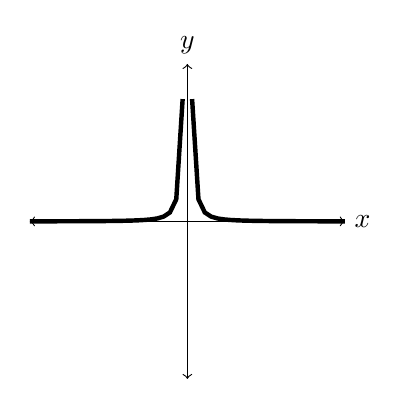
\begin{tikzpicture}[scale=0.2]
        \draw[<->] (-10,0) -- (10,0);
        \node[right] at (10,0) {$x$};
        \draw[<->] (0,-10) -- (0,10);
        \node[above] at (0,10) {$y$};
        \draw[ultra thick, domain=-10:-0.3] plot(\x, {0.7/(\x*\x)});
        \draw[ultra thick, domain=10:0.3] plot(\x, {0.7/(\x*\x)});
    \end{tikzpicture}
    \caption{$V_2$; note the singular behavior}
    \label{4.28.V2}
\end{figure}

We note that this singular $V_2$ arises because $W'$ is singular, so this doesn't work. Let's now define a new $W'(x)$ that is defined piecewise, to resolve this singularity. For $x < 0$ we will take the $W'$ that is singular at $x_0 > 0$ and for $x > 0$ we will take the $W'$ that is singular at $-x_0 < 0$, so we stich together two $W'$s. This looks like \ref{4.28.newW}
\begin{figure}[!h]
    \centering
    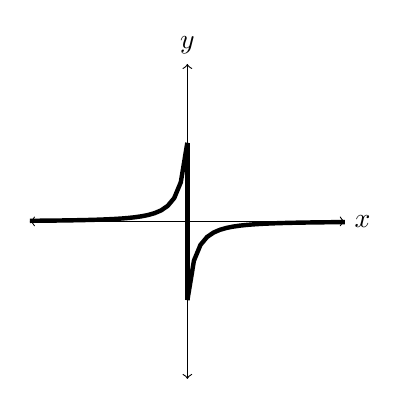
\begin{tikzpicture}[scale=0.2]
        \draw[<->] (-10,0) -- (10,0);
        \node[right] at (10,0) {$x$};
        \draw[<->] (0,-10) -- (0,10);
        \node[above] at (0,10) {$y$};
        \draw[ultra thick, domain=-10:0] plot(\x, {5/( (\x - 1)*(\x - 1))});
        \draw[ultra thick, domain=10:0] plot(\x, {-5/( (\x + 1)*(\x + 1))});
        \draw[ultra thick] (0,-5) -- (0,5);
    \end{tikzpicture}
    \caption{New $W'$ that produces a delta function}
    \label{4.28.newW}
\end{figure}

Then it is clear that $W'' \propto \delta(x)$, and since everywhere else the function looks exactly the same as our earlier $W'$ we note that it must anish everywhere $x \neq 0$, so we have our correct $V_1$.

We can then examine $V_2$ and we find that it looks like a ``volcano'' with a function that behaves a bit like $\frac{1}{x^2}$ but has a dip in the middle fixed by the delta function. This looks like \ref{4.28.volcano}
\begin{figure}[!h]
    \centering
    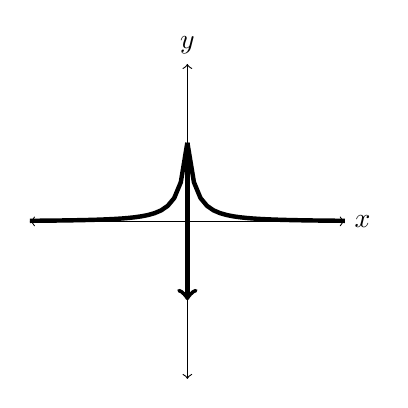
\begin{tikzpicture}[scale=0.2]
        \draw[<->] (-10,0) -- (10,0);
        \node[right] at (10,0) {$x$};
        \draw[<->] (0,-10) -- (0,10);
        \node[above] at (0,10) {$y$};
        \draw[ultra thick, domain=-10:0] plot(\x, {5/( (\x - 1)*(\x - 1))});
        \draw[ultra thick, domain=10:0] plot(\x, {5/( (\x + 1)*(\x + 1))});
        \draw[ultra thick, <-] (0,-5) -- (0,5);
    \end{tikzpicture}
    \caption{Volcano form of $V_2$}
    \label{4.28.volcano}
\end{figure}

Note interestingly that our earlier example with $V_1 = A^2$ yielded a different $V_2$ form than what we found earlier. This is because $A \neq 0$ which is a crucial difference in changing the form of $V_2$.

Let's now look at the supersymmetric WKB method. Recall the WKB formula for approximate bound state energy of potential $V_1$ looks like
\begin{align}
    \int\limits_{x_i}^{x_f} \sqrt{2m(E_{n,1} - V_1(x)}\;dx &= \left( n+\frac{1}{2} \right)\hbar \pi
\end{align}
with $n\in\mathbb{N}$. Recall that $x_i, x_f$ are the points at which $V(x_i) = V_(x_f) = E_{n,1}$. 

We then want to hit this with supersymmetric $V_2$ and see how they differ. We will expand the left hand side integral in powers of $\hbar$
\begin{align}
    \int\limits_{x_i}^{x_f}\sqrt{2m(E_{n,1} - W'^2 + \frac{\hbar}{\sqrt{2m}}W''}\;dx &= \int\limits_{x_i}^{x_f}\sqrt{2m(E_{n,1} - W'^2)}\;dx + \frac{\hbar}{2}\int\limits_{x_i}^{x_f}\frac{W''}{\sqrt{E_{n,'} - W'^2}}\;dx + O(\hbar^2)\\
    &= \int\limits_{x_i}^{x_f}\sqrt{2m(E_{n,1} - W'^2)}\;dx + \left[ \frac{\hbar}{2}\arcsin \frac{W'}{\sqrt{E_{n,1}}} \right]_{x_i}^{x_f} + O(\hbar^2)\\
\end{align}

Then up to $O(\hbar^0)$ we find $E_{n,1} = W'(x_i)^2 = W'(x_f)^2$ so the potential is determined up to lowest order by $W'$. We can then take a square root and find $\sqrt{E_{n,1} } = W'(x_f) = -W'(x_0)$ where we recall the specific choice of sign because $W'$ must be odd and $W(x > 0) > 0$ in order for our states (namely ground state $\psi_0 \propto e^{-W}$ I think) to be normalizable. We can then plug these in to the $\arcsin$ term and find
\begin{align}
    \left[ \frac{\hbar}{2}\arcsin \frac{W'}{\sqrt{E_{n,1}}} \right]_{x_i}^{x_f} + O(\hbar^2) &= \frac{\hbar \pi}{2}
\end{align}

We note that $V_1 \approx V_2$ for $\hbar \to 0$ as mentioned above, because $W'$ alone governs $\hbar^0$ behavior. This is a consequence of the WKB input and our subsequent work, which put together states that
\begin{align}
    V_1 &= \int\limits_{x_i}^{x_f}\sqrt{2m(E_{n,1} - W'(x)^2}\;dx + \frac{\hbar \pi}{2}\\
    V_2 &= \int\limits_{x_i}^{x_f}\sqrt{2m(E_{n,1} - W'(x)^2}\;dx - \frac{\hbar \pi}{2}
\end{align}

If we then put WKB ($\int \dots = (n + 1/2)\hbar \pi$) then
\begin{align}
    V_1 &= \int\limits_{x_i}^{x_f}\sqrt{2m(E_{n,1} - W'(x)^2}\;dx + \frac{\hbar \pi}{2} = \left( n + \frac{1}{2} \right)\hbar\pi & V_2 &= \int\limits_{x_i}^{x_f}\sqrt{2m(E_{n,1} - W'(x)^2}\;dx - \frac{\hbar \pi}{2} = \left( n + \frac{1}{2} \right)\hbar \pi\\
    &= n \hbar \pi & &= (n+1) \hbar \pi
\end{align}

Hey look, the supersymmetric potential is just offset by one extra energy level. This looks oddly familiar, and indeed it agrees with our earlier result!
\chapter{4/30/14 --- Total derivatives, Ahranov-Bohm effect}

We first look into some stuff we covered at the very end of 125b, namely the things about total derivatives and the \emph{Ahranov-Bohm effect}. Recall that the Lagrangian can look something like $L = \frac{mx^2}{2} + \theta \dot{x}$ with constant $\theta$ such that in the E-L equations it falls out
\begin{equation}
    \rd{}{t}\left( \pd{L}{\dot{x}} \right) - \pd{L}{x} = 0
\end{equation}
because $\rd{}{t}(\theta) = 0$ as $\theta$ is constant. Let's write this $\theta \dot{x}$ more generally as some $\Delta L$ that looks like $\dot{x}f'(x)$.because under the equations of motion this term yields a contribution $\rd{}{t}f'(x)$ which vanishes. Moreover, its contribution to the action $\Delta S = \int dt\; \Delta L$ is just $f(x)$ evaluated at the endpoints, which is constant across all paths and thus does not contribute to dynamics.

Quantum mechanically we have our propagator
\begin{align}
    U &= \bra{x_f}e^{-iHt/\hbar}\ket{x_i}\\
    &= \int [dx] \exp\left\{ \frac{i}{\hbar}\int dt\; L_0 + \frac{i}{\hbar}\left( f(x(t_f)) - f(x(t_i)) \right) \right\}\\
    &= U_0\exp\left\{ \frac{i}{\hbar}\left( f(x_f) - f(x_i) \right) \right\}
\end{align}
with $U_0$ the propagator for $L_0$. We might worry then that this total derivative changes the dynamics, but it is clear that it just adds a constant phase to everything which doesn't change dynamics. Moreover, when we change basis from the $x$ basis we can just redefine our kets to include the phase shift. This is all kind of fast because this should be review.

This hints at something bigger though; we can construct a larger set of invariances on the Lagrangian, beyond symmetries and supersymmetries, because Lagrangians that are solutions to some theory are always solutions up to a total derivative! 

We can examine this in the context of electromagnetism, trying to construct invariants. We have our four Maxwell equations
\begin{align}
    \vec{\nabla} \cdot \vec{E} &= 4\pi \rho & \vec{\nabla} \times \vec{E} + \frac{1}{c}\pd{\vec{B}}{t} &= 0\\
    \vec{\nabla} \cdot \vec{B} &= 0 & \vec{\nabla} \times \vec{B} - \frac{1}{c}\pd{\vec{E}}{t} &= \frac{4\pi}{c}\vec{J}
\end{align}

We start with $\vec{\nabla} \cdot \vec{B} = 0$ and note that this implies $\vec{B} = \vec{\nabla} \times \vec{A}$ existence of a vector potential. We can also write 
\begin{equation}
    \vec{\nabla} \times \vec{E} + \frac{1}{c}\pd{\vec{B}}{t} = \vec{\nabla} \times \underbrace{\left( \vec{E} + \frac{1}{c}\pd{\vec{A}}{t} \right)}_{-\vec{\nabla}\phi}
\end{equation}
and we can define the electromagnetic potential $\phi$, because curls of gradients vanish.

Last sort of invarinace that we have is gauge invariance, whereby we can shift $\vec{A} \to \vec{A} - \vec{\nabla} \Lambda(x,t)$ and $\phi \to \phi + \frac{1}{c}\pd{\Lambda}{t}$ and both $\vec{E}, \vec{B}$ are unchanged. The reason that this is a lot bigger than a lot of people realize is because it's invariant up to a function and not a scalar, so infinite-dimensional invariance of a sort. 

We typically choose to fix this $\Lambda$, this gauge, by some constraint. We typically choose tho Coulomb gauge $\vec{\nabla} \cdot \vec{A} = 0$. 

This has all been classical discussion; what happens in QM? We will begin with the Lagrangian
\begin{equation}
    L = \frac{1}{2}m\dot{x}^2 + \frac{q}{c}\pd{\vec{x}}{t}\cdot \vec{A} - q\phi
\end{equation}

This is then just the general EM Lagrangian. What if we undergo a gauge transformation? This takes us to
\begin{align}
    L &= L_0 - \frac{q}{c}\rd{\vec{x}}{t} - \frac{q}{c}\pd{\Lambda}{t}\\
    &= L_0 - \frac{q}{c}\rd{}{t}\Lambda
\end{align}
so it changes by a total derivative! This is very important because we already know the effect of total derivatives on the propagator. Thus, if we indeed compute the propagator we find
\begin{align}
    U\to U_0\exp\left\{ -\frac{it}{\hbar c} \right\}
\end{align}
and so our kets are just shifted by a constant phase.

{\small Aside. We can talk a little bit about how gauge invariance arises. The modern viewpoint is that gauge invariance is a natural consequence of requiring the $\vec{E}, \vec{B}$ fields to be Lorentz invariant. That is, if we construct 4-vector $(\phi, \vec{A})$ and require this to be Lorentz invariant then gauge invariance will crop up out of necessity. (Something like how relativistically we can't exhibit a fully local Hamiltonian so we need an additional freedom that is satisfied exactly by the gauge invariance? I think that's what he said).}

On that note, we can discuss the \emph{Ahranov-Bohm effect}. So the typical setup for this is to start with the two-slit experiment with some source sending charged particles through the slits onto some screen that measures impacts. Then for each point on the screen there are two paths, one through each slit, so $\psi(\vec{r}) = \psi_1(\vec{r}) + \psi_2(\vec{r})$ the amplitude at each point is the sum of the wavefunctions through each path. Fair.

We will now add a $\vec{B}$ field that does not intersect any of these paths. I will try to draw this in \ref{4.30.AB}
\begin{figure}[!h]
    \centering
    \begin{tikzpicture}[scale=0.5]
        \filldraw(-8,0) circle(0.8pt);
        \node[left, above] at (-8,0) {Source};
        \draw[ultra thick] (0,5) -- (0,2.3);
        \draw[ultra thick] (0,2) -- (0,-2);
        \draw[ultra thick] (0,-5) -- (0,-2.3);
        \draw[thick] (8,5) -- (8,-5);
        \node[right] at (5,5) {Screen};
        \draw[dashed, ->] (-8,0) -- (0,2.2);
        \draw[dashed, ->] (0,2.2) -- (8,0);
        \node[above] at (-3,1.7) {$P_1$};
        \draw[dashed, ->] (-8,0) -- (0,-2.2);
        \draw[dashed, ->] (0,-2.2) -- (8,0);
        \node[below] at (-3,-1.7) {$P_2$};
        \draw(1.5,0) circle(25pt);
        \node at (1.5,0) {{\tiny $\vec{B} \neq 0$}};
    \end{tikzpicture}
    \caption{Ahranov-Bohm setup}
    \label{4.30.AB}
\end{figure}

Classically, since our path doesn't intersect the field, it shouldn't affect dynamics. But quantum mechanically we see otherwise. Our Lagrangian becomes
\begin{equation}
    L = \frac{1}{2}m\left( \rd{\vec{r}}{t} \right)^2 + \frac{q}{c}\rd{\vec{r}}{t}\cdot \vec{A}
\end{equation}
which means then that our $\psi_1$ gets extra phase (hopefully it won't get confusing if we notate $\phi$ the phase)
\begin{equation}
    e^{i\Delta \phi} = \exp\left\{ \frac{iq}{\hbar c}\int\limits_{P_1} dt\; \rd{\vec{r}}{t}\cdot \vec{A} \right\} = \exp\left\{ \frac{iq}{\hbar c} \int\limits_{P_1}^{}d\vec{r}\cdot \vec{A} \right\}
\end{equation}
and likewise for $\psi_2$ getting extra phase $\exp\left\{ \frac{iq}{\hbar c}\int\limits_{P_2}^{}d\vec{r} \cdot \vec{A} \right\}$. Then the total phase difference looks like (we can pull out an overall phase factor)
\begin{equation}
    \Delta \phi = \frac{q}{c\hbar}\left[ \int\limits_{P_1}^{}d\vec{r} \cdot \vec{A} - \int\limits_{P_2}^{}d\vec{r} \cdot \vec{A} \right]
\end{equation}

But then we note that paths $P_1, P_2$ form a closed path if we flip the sign of $P_2$ (perhaps more evident if we consult the disgustingly beautiful \ref{4.30.AB}), so the phase shift actually can be written
\begin{equation}
    \Delta \phi = \frac{q}{c\hbar} \oint\limits_{P_1, P_2} d\vec{r} \cdot \vec{A}
\end{equation}

We can then throw Stokes theorem at this and obtain
\begin{equation}
    \Delta \phi = \frac{q}{c\hbar}\int \left( \vec{\nabla} \times \vec{A} \right)\cdot d\vec{S} = \frac{q}{c\hbar}\int \vec{B} \cdot d\vec{S} = \frac{q}{c\hbar} \Phi_B
\end{equation}
with $\Phi_B$ the magnetic flux. The wavefunction then looks like
\begin{equation}
    \psi(r) = \psi_1e^{\frac{iq}{c\hbar}\Phi_B} + \psi_2
\end{equation}
\chapter{5/2/14 --- Dirac charge quantization, Finishing Ahranov-Bohm}

Recall that our phase shift in the Ahranov-Bohm effect was given $\frac{iq}{c\hbar}\Phi_m$. Then we note that if we choose $\Phi_m = n\Phi_0$ with $\Phi_0 = \frac{2\pi \hbar c}{q}$ some quantized unit of flux, we see that the Ahranov-Bohm effect is not observed because the phase shift goees to $1$.

Using this we can look into an interesting phenomenn, namely \emph{Dirac charge quantization}. We consider some long but finite solenoid with some $\vec{B}$. Of course if we choose our paths $P_1, P_2$ to be sufficiently close to the solenoid we exhibit the Ahranov-Bohm effect, because the returning flux is very small compared to the inside of the solenoid. Instead though, we can approach this setup differently, proposed by Dirac. 

Let $a$ be the radius of the solenoid. We will examine in the $a \to 0$ limit. Then the only way we can still observe the field is via the Ahranov-Bohm effect. But now this lends itself to a further condition: let's choose the solenoid's flux to be $n \Phi_0$ so that it's invisible to the Ahranov-Bohm effect. This solenoid, vanishing radius and correct quantized flux, is called the \emph{Dirac string}, is invisible. The setup now looks like a magnetic monopole, because the solenoid is gone. Now if we choose a sufficiently long solenoid, we have a mangetic monopole in isolation.

If we are to accomodate for this monopole in Maxwell's equations, we must examine $\vec{\nabla} \cdot \vec{B} = 0$. If we have magnetic monopoles, then this must become $\vec{\nabla} \cdot \vec{B} = 4\pi \rho_m \neq 0$. We can then use Gauss's Law on the Coulomb-like force $\vec{B} = \frac{q_m \hat{r}}{r^2}$. We note that the flux resulting from this must look like $\Phi_m = 4\pi q_m$. But then since this monopole doesn't really exist because of the Dirac string, we note that this flux from the monopole must cancel with the quantized $\Phi_B$ from the Dirac string, producing condition
\begin{equation}
    \frac{2q_m q}{c\hbar} = n
\end{equation}
with $q$ the electric charge. Then the electric and magnetic charges must be quantized with respect to one another. Note that this doesn't show show that $q$ itself is quantized to anything in particular, but the only way to exhibit a monopole consistent with Maxwell equations is to quantize it with respect to fundamental electric charge. 

Now let's actually compute something with the Ahranov-Bohm. Let's exhibit a particle travelling around a ring of radius $b$ with a coaxial solenoid of radius $a$ in the middle with field $B\hat{z}$. The Ahranov-Bohm effect is in here; we see the two paths are going one way as opposed to the other way around the ring. To do anything quantum mechanical we will need the Lagrangian/Hamiltonian, which requires $\vec{A}$. This can be written down (we can check this on our own)
\begin{equation}
    \vec{A} = 
    \begin{cases}
        \hat{\phi} \frac{\Phi_m r}{2\pi a^2} & r < a\\[10pt]
        \hat{\phi} \frac{ \Phi_m}{2\pi r} & r > a
    \end{cases}
\end{equation}
with $\Phi_m = B\pi a^2$. We should also set $\phi = 0$ the electric potential. This gives Lagrangian and Hamiltonian
\begin{align}
    L &= \frac{1}{2}m\left( \rd{\vec{r}}{t} \right)^2 + \frac{q}{c}\rd{\vec{r}}{t}\cdot\vec{A}\\
    H &= \frac{\left( \vec{p} - \frac{q}{c}\vec{A} \right)^2}{2m}\\
    &= \frac{1}{2m}\left[ -i\hbar\vec{\nabla} - \frac{q}{c}\vec{A} \right]^2
\end{align}
going into coordinate basis. Note that $\vec{A}$ is a function of $\vec{r}$ so these don't commute. We will thus have to square more carefully
\begin{align}
    H &= \frac{1}{2m}\left[ -\hbar^2 \vec{\nabla}^2 + \frac{q^2}{c^2}\vec{A}^2 + \frac{2i\hbar q}{c}\vec{A} \cdot \vec{\nabla} \right]
\end{align}
(note that there was a $\vec{\nabla} \vec{A}$ term that commutes to $\vec{A} \vec{\nabla}$ under Coulomb gauge; these are not dot products but products of operators! This tripped everybody (including Cliff) up for some time). Note that $\psi = \psi(\phi)$ only by symmetries/constraints, so we can write down Hamiltonian
\begin{align}
    H \psi_E = E\psi_E &= \frac{1}{2m}\left[ -\frac{\hbar^2}{b^2}\rtd{}{\phi} + \left(\frac{q\Phi_m}{2\pi b x}\right)^2 + \frac{i\hbar q}{\pi b^2}\frac{\Phi_m}{c}\rd{}{\phi} \right]\psi_E
\end{align}

This is then just an ODE, but we go ahead and define some quantities to help us out $\beta = \frac{q \Phi_m}{2\pi \hbar c}, \epsilon = \frac{2mb^2E}{\hbar^2} - \beta^2$ (replacements for the magnetic field/energy) which turns us into
\begin{align}
    \rtd{\psi_E}{\phi} - 2i\beta \rd{\psi_E}{\phi} + \epsilon\psi_E &= 0
\end{align}

We know physically that $\psi_E = Ae^{in\phi}$ with integer $n$ because we are on a ring. If we plug this ansatz in, we find
\begin{align}
    -n^2 + 2\beta n + \epsilon &= 0\\
    n &= \beta \pm \sqrt{\beta^2 + \epsilon}\\
    &= \beta \pm \frac{b}{\hbar}\sqrt{2mE}
\end{align}
which quantizes the energies at last! This gives
\begin{equation}
    \boxed{E_n = \frac{\hbar^2}{2mb^2}\left( n - \frac{q\Phi_m}{2\pi\hbar c} \right)^2}
\end{equation}

The best way to understand this is to compare to a particle on a ring without $\vec{B}$, so $\Phi_m \to 0$. This then looks like \ref{5.2.plot}
\begin{figure}[!h]
    \centering
    \begin{tikzpicture}[scale=0.4]
        \draw[<->] (-10,0) -- (10,0);
        \node[right] at (10,0) {$n$};
        \draw[<->] (0,0) -- (0,10);
        \node[above] at (0,10) {$E$};
        \draw[dashed, domain=-5:5] plot(\x, {\x*\x/2.5});
        \draw (-5.3, 10) -- (-4.7,10);
        % \draw (-4.3, 6.4) -- (-3.7,6.4);
        \draw (-3.3, 3.6) -- (-2.7,3.6);
        % \draw (-2.3, 1.6) -- (-1.7,1.6);
        \draw (-1.3, 0.4) -- (-0.7,0.4);
        \draw (5.3, 10) -- (4.7,10);
        % \draw (4.3, 6.4) -- (3.7,6.4);
        \draw (3.3, 3.6) -- (2.7,3.6);
        % \draw (2.3, 1.6) -- (1.7,1.6);
        \draw (1.3, 0.4) -- (0.7,0.4);
        \draw[red, dashed, domain=-8:2] plot(\x, {(\x + 3)*(\x + 3)/2.5});
        \draw[red] (-8.3, 10) -- (-7.7,10);
        % \draw[red] (-7.3, 6.4) -- (-6.7,6.4);
        \draw[red] (-6.3, 3.6) -- (-5.7,3.6);
        % \draw[red] (-5.3, 1.6) -- (-4.7,1.6);
        \draw[red] (-4.3, 0.4) -- (-3.7,0.4);
        \draw[red] (1.7, 10) -- (2.3,10);
        % \draw[red] (0.7, 6.4) -- (1.3,6.4);
        \draw[red] (-0.3, 3.6) -- (0.3,3.6);
        \draw[red] (-1.3, 1.6) -- (-0.7,1.6);
        \draw[red] (-2.3, 0.4) -- (-1.7,0.4);
        \draw[blue, dashed, domain=-2.5:7.5] plot(\x, {(\x - 2.5)*(\x - 2.5)/2.5});
        \draw[blue] (-2.3, {20.25/2.5}) -- (-1.7, {20.25/2.5});
        % \draw[blue] (-1.3, {3.5*3.5/2.5}) -- (-0.7, {3.5*3.5/2.5});
        \draw[blue] (-0.3, {2.5*2.5/2.5}) -- (0.3, {2.5*2.5/2.5});
        \draw[blue] (1.7, {0.5*0.5/2.5}) -- (2.3, {0.5*0.5/2.5});
        \draw[blue] (2.7, {0.5*0.5/2.5}) -- (3.3, {0.5*0.5/2.5});
        \draw[blue] (4.7, {2.5*2.5/2.5}) -- (5.3, {2.5*2.5/2.5});
        \draw[blue] (6.7, {20.25/2.5}) -- (7.3, {20.25/2.5});
        \draw (-6,-0.3) -- (-6,0.3);
        \draw (-4,-0.3) -- (-4,0.3);
        \draw (-3,-0.3) -- (-3,0.3);
        \draw (-2,-0.3) -- (-2,0.3);
        \draw (-1,-0.3) -- (-1,0.3);
        \draw (5,-0.3) -- (5,0.3);
        \draw (4,-0.3) -- (4,0.3);
        \draw (3,-0.3) -- (3,0.3);
        \draw (2,-0.3) -- (2,0.3);
        \draw (1,-0.3) -- (1,0.3);
        \draw (0,-0.3) -- (0,0.3);
    \end{tikzpicture}
    \caption{Comparison of particle in a box with and without $B$ field. Note that the energy levels are where the $x$ axis is integer, as marked (only select ones marked). Black is $B = 0$, blue is $B \neq 0$, and red is $B = n\Phi_0$. Omitted some energy levels for clarity.}
    \label{5.2.plot}
\end{figure}

Note that the energy levels are only where the $x$ axis is integral, so that means that shifts usually produce really weirdly-split energy levels. However, if we shift by $n\Phi_0$ the quantum flux then we cannot observe any change in energy levels! Refer to \ref{5.2.plot} to get an idea of what happens when shifted by integer (note that the red energy levels occur at the same  $E$ as the black ones, showng that a shift by $n\Phi_0$ produces the same energy levels, but the blue ones occur at different $E$s!).

This procedure is at the root of measuring small $B$ fields. Thankfully, ACM95c is a joke so I have enough time to finish this plot after class.
\chapter{5/5/14 --- Superconductivity}

Very rich topic, we will cover cursorily. Superconductivity is phenomenon whereby at sufficiently low temperature $T$ we see that certain metals conduct without resistance. 

Consider a metal as a lattice of atoms with a sea of electrons flying around, and specifically bosonic Cooper pair superconductivity. The statement of these assumptions is then
\begin{itemize}
    \item Electrons polarizing medium will actually produce attractive forces in between each other.
    \item Then \emph{Cooper pairs} of electrons become bound, the critical assumption that changes between conductors and superconductors. Note that this pair is a bosonic state because combination of two fermions.
\end{itemize}

We will the throw QM at the wavefunction $\psi(\vec{r},t)$ of the Cooper pairs. Note then that $\psi^*\psi$ describes the charge density of the electron (or maybe the Cooper pair, so factor of $2$ might be introduced; we won't care much about this). We will call this then $\rho = \psi^*\psi$. We know by the continuity equation then that 
\begin{align}
    \pd{\rho}{t} + \vec{\nabla} \cdot \vec{J} &= 0\\
    \pd{\rho}{t} &= \pd{\psi^*}{t}\psi + \psi^* \pd{\psi}{t}
\end{align}

We know though that $\pd{\psi}{t}$ is governed by the SE, We know that this is the SE for Hamiltonian $\frac{\left(P^2 - \frac{q}{c}A\right)^2}{2m} + q\phi$, so we can plug this through our continuity equation and obtain as solution (Cliff! Don't be like Mark Wise and not show us the algebra)
\begin{equation}
    \vec{J} = \frac{1}{2}\left[ \left(\frac{-i\hbar \vec{\nabla} - \frac{q}{c}\vec{A}}{m}\psi\right)^\dagger\psi + \psi^\dagger\left( \frac{-i\hbar \vec{\nabla} - \frac{q}{c}\vec{A}}{m}\psi \right) \right]\label{5.5.J}
\end{equation}
where the $\phi$ electric potential happens to cancel out. 

We will also need to examine the freedom of a phase in our $\psi$ that isn't encapsulated in our $\rho$ definition. So let's write $\psi(\vec{r},t) = \sqrt{\rho(\vec{r},t)} e^{i\theta(\vec{r},t)}$. Plugging this form through and assuming spatial constantness of $\rho$ gives us unenlightening expression
\begin{align}
    \psi^\dagger\left( -i\hbar \vec{\nabla} - \frac{q}{c}\vec{A} \right)\psi &= \sqrt{\rho}e^{-i\theta}\left( \hbar \vec{\nabla}\theta e^{i\theta}\sqrt{\rho} - i\hbar \vec{\nabla}\rho \frac{1}{2\sqrt{\rho}}e^{i\theta} - \frac{q\vec{A}}{c}\sqrt{\rho}e^{i\theta} \right)\\
    &= \rho\left[ \hbar \vec{\nabla}\theta - i\hbar\frac{\vec{\nabla}\rho}{2\rho} - \frac{q}{c}\vec{A} \right]
\end{align}

We can then plug this back into \eqref{5.5.J} to obtain
\begin{align}
    \vec{J} &= \frac{\hbar}{m}\rho\left[ \vec{\nabla}\theta - \frac{q}{\hbar c}\vec{A} \right]
\end{align}

We can then plug this back through our continuity equation again and obtain
\begin{equation}
    \pd{\rho}{t} = 0 = \vec{\nabla} \cdot \vec{J} = \frac{\hbar \rho}{m}\left( \nabla^2 \theta - \frac{q}{\hbar c}\vec{\nabla} \cdot \vec{A} \right)
\end{equation}
where we go ahead and assume $\rho$ is negative so the charge continuity equation flips. We also assume electrostatics as evident above. We then note that if we were in the Coulomb gauge that $\nabla^2 \theta = 0$ for which a solution is $\theta$ constant so we choose $0$. Then we finally find
\begin{equation}
    \vec{J} = -\frac{\rho q}{mc}\vec{A}
\end{equation}

Plugging this into Maxwell equations gives, assuming Coulomb gauge again (define $\Box^2 = \frac{1}{c^2}\ptd{}{t} - \nabla^2$ the \emph{d'Alembertian})
\begin{align}
    \Box^2 \vec{A} + \vec{\nabla} \cdot \left( \left( \vec{\nabla} \cdot \vec{A} \right) + \frac{1}{c^2}\pd{\phi}{t} \right) &= \mu_0 \vec{J}\\
    \Box^2 \vec{A} &= -\frac{\mu_0 \rho q}{mc}\vec{A}\\
    (\Box^2 + \lambda^2) \vec{A} &= 0
\end{align}
where we define $\lambda^2 \equiv \frac{\mu_0 \rho q}{mc}$. Note that this is very different from the typical wave equations because there's a homogeneous term in the wave equation now, namely the $\lambda^2 \vec{A}$. Then this looks like giving photon an effective mass $\lambda^2$!

We know that solutions look like $\vec{A} \sim e^{\pm \lambda x}$ which gives $\vec{E}, \vec{B} \sim e^{\pm \lambda x}$. Then if a wave is incoming and hits the superconductor, boundary conditions aside the plane wave must turn into an exponential decay solution, as the exponential growth $e^{\lambda x}$ is unphysical. So it would look something like \ref{5.5.conductorGraph}
\begin{figure}[!h]
    \centering
    \begin{tikzpicture}[scale=0.5]
        \draw[<->] (-10,0) -- (10,0);
        \node[right] at (10,0) {$x$};
        \draw[<->] (0,-2) -- (0,10);
        \node[above] at (0,10) {$\vec{E}$};
        \draw[red, domain=0:8] plot(\x, {3*sin(\x*62.8) + 4});
        \node[above] at (5,7) {Incoming Wave};
        \draw[blue, domain=-8:0] plot(\x, {4*exp(\x)});
        \node[above] at (-5,3) {Superconductor};
    \end{tikzpicture}
    \caption{Entry of a wave into superconductor.}
    \label{5.5.conductorGraph}
\end{figure}

The characteristic attentuation depth of the decaying field is called the London penetration depth, goes with $\frac{1}{\lambda}$. We are leaving out a lot of factors, so this isn't an exact result, but we do know that incoming waves must indeed attenuate.

This gives rise to the Meissner effect. Consider a solid conductor. Then at large $T$ (temperature) it allows $\vec{B}$ fields while at small $T$ it expels the fields so the fields go around. But let's try a conductor that looks like an annulus. The large $T$ case still looks the same $\vec{B}$ everywhere. But in the small $T$ case, there are some field lines that run through the middle of the annulus, but nothing going through the annulus. Then if we suddenly shut off the $\vec{B}$ field, the field that goes through the middle of the cylinder cannot die off, because it would require some field lines to go \emph{through} the annulus to cancel it out! Thus the field lines outside the cylinder wrap back around, such that we obtain a trapped $\vec{B}$ flux. 

\chapter{5/7/14 --- Flux quanta, confinement, Josephson Junctions}

Let's recap what we saw last time. Recall that we found that the superconducting torus trapped $\vec{B}$ field. Moreover, we found the following equations
\begin{align}
    \psi &= \sqrt{\rho}e^{i\theta}\\
    \vec{J} = 0 &= \frac{\hbar}{m}\rho\left[ \vec{\nabla} \theta - \frac{q}{\hbar c}\vec{A} \right]\\
    \frac{\hbar c}{q}\vec{\nabla} \theta &= \vec{A}\\
    \frac{\hbar c}{q} \oint\limits_C \vec{\nabla} \theta d\vec{s} &= \oint\limits_C \vec{A} \cdot d\vec{s}
\end{align}

We can evaluate these explicitly. We note that the left hand side should be an integral over an exact differential and so vanish, but we will leave it in terms of $\theta_2, \theta_1$ endpoints for now (these should be equal given closed surface of integration). This gives
\begin{align}
    \frac{\hbar c}{q}(\theta_2 - \theta_1) &= \int\limits_{S}^{}\vec{\nabla} \times \vec{A}\cdot d\vec{n}\\
    &= \int\limits_{S}^{}\vec{B}\cdot d\vec{n} = \Phi_m
\end{align}
the magnetic flux. This then seems to yield that $\Phi_m$ is vanishing, but we'll use a loophole. We recall that $\theta_i$ is a periodic variable however, so $\theta_2 - \theta_1 = 2\pi n$ is all that is required; this is also evident from $\psi(\theta) \propto e^{i\theta}$. This then again quantizes the flux, and so we find
\begin{align}
    \Phi_m = \frac{2\pi \hbar c n}{q}
\end{align}

Thus if we are inclined to think of field lines as being physical, then each field line can correspond to a single quantum flux of field, in some intuitive sense. Note also that these flux quanta are very measurable indeed, much more so than mechanical ones!

Intuitively we can think of charge quantization as a property of angular momentum. Suppose that we start with a magnetic monopole, then it turns out that if we throw an electron at it the electron's only change is in its angular momentum! We also know that angular momentum is quantized from quantum mechanics, so we also find another co-quantization condition on electric/magnetic charge.

Let's now smash magnetic monopoles and superconductors together. Suppose we have some superconducting material at room temperature inside of which we put two magnetic monopoles (effectively a magnet). We then know that the $\vec{B}$ lines exit one monopole and enter the other. To be formal, let's draw Dirac strings on each monopole connected to other monopoles very very far away (let these two monopoles not be connected). 

Then if we let the temperature fall, all magnetic field lines should damp exponentially inside the material by what we discussed earlier. It turns out that the resulting field geometry looks like a very thin and packed ``flux tube'' connecting the two monopoles (not to be confused with Dirac string). Let's examine the properties of this flux tube. 

We can compute the energy of the flux tube to go with the product of the ``string tension'' $T$ and the length $L$ of the tube, so if the two ends are farther away then the stored energy increases linearly. This is notable since we're used to particles that interact with $L^{-1}$ but here we're interacting at $L$. So if we try to pull these monopoles really far apart, the energy of the flux strings will exceed the particle rest mass, and therefore it becomes energetically favorable for the flux string to decompose into two new monopoles (out of thin air!). This phenomenon is called ``confinement.''

This is very similar to quarks; we recall that the proton is comprised of two $u$ quarks and one $d$ quark, charges $\frac{2}{3}, -\frac{1}{3}$ respectively. The reason that we cannot see quarks independently (and never observe fractional charge) is because again confinement generates new quarks when we try to pull quarks apart (because quark potentials go with something stronger than $r^{-1}$ as well). (It turns out that the phenomenon of \emph{asymptotic freedom} (David Politzer's Nobel prize!) arises at super high energies, where the quark-interaction actually goes down to $r^{-1}$ at sufficiently high energies, and so confinement fails and we can observe bare quarks.)

We lastly look into Josephson Junctions (apparently he's really crazy; Cliff says ``this may be one of the rare cases where a Nobel laureate has done more harm than good for science.''). Let's now look at two superconductors separated by an insulator. Then within each conductor we have the wavefunctions we've already examined, so we can write for the full system
\begin{align}
    \ket{\psi} &= \begin{pmatrix} \ket{\psi_1}\\ \ket{\psi_2} \end{pmatrix} & H &= \begin{pmatrix} U_1 & K \\ K & U_2 \end{pmatrix} 
\end{align}
with $U_i$ the energies of the individual systems and $K$ some interaction coupling energy. We can then write down SEs
\begin{align}
    i\hbar \pd{\psi_1}{t} &= U_1\psi_1 + K\psi_2 & i\hbar \pd{\psi_2}{t} &= U_2\psi_2 + K\psi_1
\end{align}

Let's now put a voltage difference between the two superconductors. Then we know that $U_1 - U_2 = qV$, and we can zero the energies to rewrite our SEs
\begin{align}
    i\hbar \pd{\psi_1}{t} &= \frac{qV}{2}\psi_1 + K\psi_2 & i\hbar \pd{\psi_2}{t} &= -\frac{qV}{2}\psi_2 + K\psi_1
\end{align}
with wavefunctions $\psi_1 = \sqrt{\rho_1}e^{i\theta_1}, \psi_2 = \sqrt{\rho_2}e^{i\theta_2}$. We then want to solve for $U_i, K$ in terms of $\rho_i, \theta_i$. We plug into our SE and obtain
\begin{align}
    \dot{\rho}_1 = \dot{\rho}_2 &= \frac{2}{\hbar}K\sqrt{\rho_1\rho_2}\sin \delta\\
    \dot{\theta}_1 &= \frac{K}{\hbar}\sqrt{\frac{\rho_2}{\rho_1}}\cos\delta - \frac{qV}{2\hbar}\\
    \dot{\theta}_2 &= \frac{K}{\hbar}\sqrt{\frac{\rho_1}{\rho_2}}\cos\delta + \frac{qV}{2\hbar}
\end{align}
with $\delta = \theta_2 - \theta_1$. Then the dynamics only depend on $\delta$ the phase difference, which is what we expect. We will continue this next lecture.
\chapter{5/9/14 --- More Josephson Junctions}

We can examine the current flowing through the Josephson junction to be
\begin{equation}
    J = \dot{\rho}_1 - \dot{\rho}_2 = \frac{2}{\hbar}K\sqrt{\rho_1\rho_2} \sin \delta
\end{equation}
with of course $\delta = \theta_2 - \theta_1$. We also know
\begin{align}
    \dot{\theta_1} &= \frac{k}{\hbar}\sqrt{\frac{\rho_2}{\rho_1}}\cos\delta - \frac{qV}{2\hbar} & \dot{\theta_2} &= \frac{k}{\hbar}\sqrt{\frac{\rho_1}{\rho_2}}\cos\delta + \frac{qV}{2\hbar}
\end{align}

We will further more assume that $\rho_1 = \rho_2$ constant, i.e. the two superconductors are actually connected or something. This allows us to say that there is nonvanishing current but that the $\rho$ are still constant. Then we can write
\begin{equation}
    J(t) = \frac{2k\rho_0}{\hbar}\sin \delta(t) = J_0\sin\left(\delta_0 + \frac{q}{\hbar}\int\limits^t V\; dt\right)
\end{equation}
as $\dot{\theta}_2 - \dot{\theta}_1 = \frac{qV}{\hbar}$. This shows that the phase of the current goes with
\begin{equation}
    \delta(t) = \delta_0 + \frac{q}{\hbar}\int\limits_{}^{t}V(t')\;dt'
\end{equation}

Let's see what this tells us. Note that the integral is actually the classical term, because it goes with $\hbar^{-1}$. So if we give the current some constant current $V$, then we see that the current goes approximately to $0$ in the time average, which makes sense since we're putting an insulator in the middle.

We see the quantum mechanical effect by setting $V(t) = 0$. Then we still see that there is some current, driven by this $\sin\delta_0$ amplitude! This is the quantum mechanical effect; if you let two superconductors sit on either side then charge tunnels across and forms a current.

Let's now look at a double Josephson Juction with a $\vec{B}$ field in the middle, as in \eqref{5.9.JJ}
\begin{figure}[!h]
    \centering
    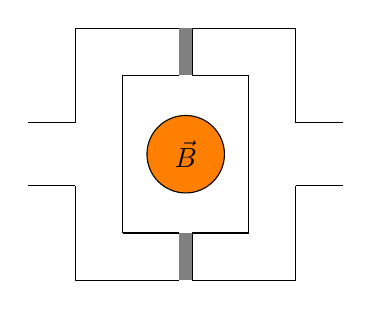
\begin{tikzpicture}[scale=0.2]
        \draw (-10,2) -- (-7,2);
        \draw (-7,2) -- (-7,8);
        \draw (-7,8) -- (-0.4,8);
        \draw (-0.4,8) -- (-0.4,5);
        \draw (-0.4,5) -- (-4,5);
        \draw (-4,5) -- (-4,-5);
        \draw (4,5) -- (4,-5);
        \draw (10,2) -- (7,2);
        \draw (7,2) -- (7,8);
        \draw (0.4,8) -- (0.4,5);
        \draw (0.4,5) -- (4,5);
        \draw (7,8) -- (0.4,8);
        \draw (-10,-2) -- (-7,-2);
        \draw (-7,-2) -- (-7,-8);
        \draw (-7,-8) -- (-0.4,-8);
        \draw (-0.4,-8) -- (-0.4,-5);
        \draw (-0.4,-5) -- (-4,-5);
        \draw (10,-2) -- (7,-2);
        \draw (7,-2) -- (7,-8);
        \draw (0.4,-8) -- (0.4,-5);
        \draw (0.4,-5) -- (4,-5);
        \draw (7,-8) -- (0.4,-8);
        \filldraw[orange, draw=black] (0,0) circle(70pt);
        \node at (0,0) {$\vec{B}$};
        \fill[gray] (-0.4,5) rectangle(0.4,8);
        \fill[gray] (-0.4,-5) rectangle(0.4,-8);
    \end{tikzpicture}
    \caption{Double Josephson Junction. Grey sections are insulators, orange (woohoo, color!) is the magnetic field.}
    \label{5.9.JJ}
\end{figure}

This is then obviously an Ahranov-Bohm effect. The phase shift along $S_1 = \delta_1 + \frac{q}{\hbar c}\int\limits_{C_1}\vec{A} \cdot d\vec{r}$ and correspondingly along $S_2 = \delta_1 + \frac{q}{\hbar c}\int\limits_{C_2}\vec{A} \cdot d\vec{r}$. Then we know Ahranov-Bohm must produce $\delta_2 - \delta_1 = \frac{q}{\hbar c}\Phi_m$. Let's then write for convenience $\delta_0 = \frac{\delta_1 + \delta_2}{2}$. Then the total current that runs through the Josephson Junction looks like
\begin{align}
    J_{tot} &= J_1 + J_2 = J_0\sin \delta_1 + J_0\sin \delta_2\\
    &= J_0\left[ \sin\left( \delta_0 - \frac{q}{2\hbar c}\Phi_m \right) + \sin \left( \delta_0 + \frac{q}{\hbar c}\Phi_m \right) \right]\\
    &= 2J_0\sin \delta_0 \cos\left( \frac{q}{2\hbar c}\Phi_m \right)
\end{align}

Note that the Josephson Junction is what allows us to measure the $\vec{B}$ field in the middle; without this we would not measure any current! (I think this is the punch line?)

This result is realy cool because it allows measurement of really weak magnetic fields! The above Josephson Junctions are called \emph{SQUIDs} or \emph{superconducting quantum interference device}. It is actually possible in magnetocenphalography to use these SQUIDs to measure magnetic fields down to $10^{-15}\mathrm{T}$! We can then study brain waves using this.

We're going to completely shift gears now, to model a crystal. Consider a potential within a cell to look like
\begin{equation}
    V(x) =
    \begin{cases}
        V_0 & -b < x < 0\\
        0 & 0 < x < a
    \end{cases}
\end{equation}
and we repeat every $c = a+b$ down the line. There are then infinitely many barriers, like in \eqref{5.9.barriers}
\begin{figure}[!h]
    \centering
    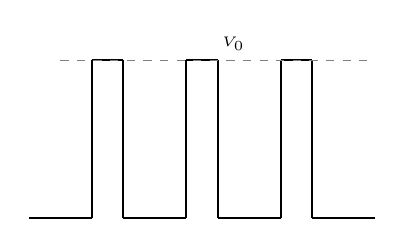
\begin{tikzpicture}[scale=0.2]
        \draw[thick] (-12,0) -- (-8,0);
        \draw[thick] (-6,0) -- (-2,0);
        \draw[thick] (0,0) -- (4,0);
        \draw[thick] (6,0) -- (10,0);
        \draw[thick](-8,0) -- (-8,10);
        \draw[thick] (-8,10) -- (-6,10);
        \draw[thick](-6,0) -- (-6,10);
        \draw[thick](0,0) -- (0,10);
        \draw[thick] (-2,10) -- (-0,10);
        \draw[thick](-2,0) -- (-2,10);
        \draw[thick](4,0) -- (4,10);
        \draw[thick] (4,10) -- (6,10);
        \draw[thick](6,0) -- (6,10);
        \draw[gray, dashed] (-10,10) -- (10,10);
        \node[above] at (1,10) {{\tiny $V_0$}};
    \end{tikzpicture}
    \caption{Crystal Potential Barrier; width of each nub is $b$, each ``down'' section is $a$.}
    \label{5.9.barriers}
\end{figure}.

We then write down the general state. We know it must repeat with period $c$ as well, so we write
\begin{equation}
    \psi_E(x) =
    \begin{cases}
        \psi_{1E}(x) & 0 < x < a\\
        \psi_{2E}(x) & -b < x < 0
    \end{cases}
\end{equation}

Then we have time-independent SEs
\begin{align}
    \rtd{\psi_{1E}}{x} + \frac{2mE}{\hbar^2}\psi_{1E} &= 0 & \rtd{\psi_{2E}}{x} + \frac{2m(E - V_0)}{\hbar^2}\psi_{2E} &= 0
\end{align}
which yields general forms
\begin{align}
    \psi_{1E} &= A_1e^{ik_1x} + B_1e^{-ik_1x} & \psi_{2E} &= A_1e^{ik_2x} + B_1e^{-ik_2x}
\end{align}
for $k_1 = \frac{\sqrt{2mE}}{\hbar}, k_2 = \frac{\sqrt{2m(E-V_0)}}{\hbar}$. We will finish this next lecture. Next time we'll take these equations given the periodicity of the system and show a straightforward solution. 

\chapter{5/12/14 --- Crystals}

Recall the periodic potential we used to model the potential, depicted in \ref{5.9.barriers}; repeating square wells of height $V_0$. We then took the forms of our wavefunctions to be
\begin{align}
    \psi_{1E} &= A_1e^{ik_1x} + B_1e^{-ik_1x} & \psi_{2E} &= A_1e^{k_2x} + B_1e^{-k_2x}\label{5.12.eigens}
\end{align}
with $k_1 = \frac{\sqrt{2mE}}{\hbar}$ and $k_2 = \frac{\sqrt{2m(V_0 - E)}}{\hbar}$; note that $k_2$ was imaginary but we now made it real, because $E < V_0$ for these bound states.

Let's then examine the operator $T\psi(x) = \psi(x+c)$, which takes the state from one well to another. We note that this looks like a translation operator, which we know takes on form $T = e^{-\frac{i}{\hbar}Pc}$ which translates $\psi$ by $c$. We examine this and note that $T$ is unitary. Moreover, since the potential is translationally symmetric by $c$ we note that $[T,H] = 0$. Then let's look at
\begin{align}
    H \psi_E &= E\psi_E\\
    H(T\psi_E) &= TH\psi_E = TE\psi_E = E(T\psi_E)
\end{align}

This is like back in angular momentum; we note that eigenstates of $T$ are also eigenstates of $H$ because they commute, so we can index our eigenstates $T\psi_E = t\psi_E$ by eigenvalues as well. Moreover, since $T$ is unitary, we know that $t$ must be a pure phase $\abs{t} = 1$. Then we can write $t = e^{ikc}$ and index our eigenvalues under $T$ by $k$ instead, and we can think of $k$ as a new quantum number! Welcome to the family.

Let's put this all together. We note that $\psi_E(x+c) = e^{ikc} \psi_E(x)$ which is much easier to work with. Let's then introduce the ansatz $\psi_e(x) = u_k(x) e^{ikx}$ with $u_k(x+c) = u_k(x)$ completely translationally invariant. 

We now have the tools to solve the system. Let's introduce boundary conditions $\psi_{1E}(0) = \psi_{2E}(0), \psi_{1E}'(0) = \psi_{2E}'(0)$. Then if we just plug in our eigenfunctions from \eqref{5.12.eigens} then we find first $A_1 + B_2 = A_2 + B_2$ and then $ik_1A_1 - ik_1B_1 = k_2A_2 - k_2B_2$. We next find boundary conditions on $u_k$. First we note $u_k(a) = u_k(-b)$, so $e^{-ika}\psi_{1E}(a) = e^{ikb}\psi_{2E}(-b)$, which plugging in again eigenfunctions \eqref{5.12.eigens} gives 
\begin{equation}
    e^{-ika}\left( A_1e^{ik_1a} + B_1e^{-ik_1a} \right) = e^{ikb}\left( A_2e^{-k_2b} + B_2e^{k_2b} \right)
\end{equation}

We can of course also construct condition $u_k'(a) = u_k'(-b)$. We can just go through the algebra, but what we obtain is
\begin{align}
    \pd{}{x}\left[ e^{-ikx}\psi_{1E}(x) \right]_{x=a} &=\pd{}{x}\left[ e^{-ikx}\psi_{2E}(x) \right]_{x=-b}\\
    i(k_1 - k)A_1e^{i(k_1-k)a} - i(k_1 + k)B_1e^{-i(k_1 + k)a} &= (k_2 - ik)A_2e^{-(k_2 - ik)b} - (k_2 + ik)B_2e^{(k_2 + ik)b}
\end{align}

We could solve out these four BCs and plot the wavefunction, but this isn't too illuminating. Instead, we think that $k$ must do some sort of quantization, so we inspect its relation with energy. We will look at a shortcut. We note that for some $\mathbf{M}$ defined by our four equations above, we have
\begin{equation}
    \mathbf{M}\begin{pmatrix} A_2 \\ B_2 \\ -A_1 \\ -B_1 \end{pmatrix} =0 = \begin{pmatrix} 1 & 1 & 1 & 1\\ k_2 & -k_2 & ik_1 & -ik_1 \\ e^{(ik - k_2)b} & e^{(ik + k_2)b} & e^{i(k_2 - k)a} & e^{-i(k_1 + k)a}\\ (k_2 - ik)e^{(ik - k_2)b} & -(k_2 + ik) e^{(ik + k_2)b} & (ik_1 - k) e^{i(k_1 - k)a} & -(ik_1 + k) e^{-i(k_1 + k)a} \end{pmatrix} \begin{pmatrix} A_2 \\ B_2 \\ -A_1 \\ -B_1 \end{pmatrix}
\end{equation}

We then just take the determinant of $\mathbf{M}$ and set it equal to zero, which actually yields 
\begin{equation}
    \frac{k_2^2 - k_1^2}{2k_1k_2}\sinh(k_2b)\sin(k_1a) + \cosh k_2b \cos k_1a = \cos kc
\end{equation}

Note that $k_{1,2}$ are related to $E, V_0$ and $a,b,c$ are distances. Thus, this equation fixes $k$ with respect to $E$ energies. We moreover note that the right hand side must be bound by $\pm 1$, so let's try a plot of the left hand side as a function of $E/V_0$ in \ref{5.12.plot}
\begin{figure}[!h]
    \centering
    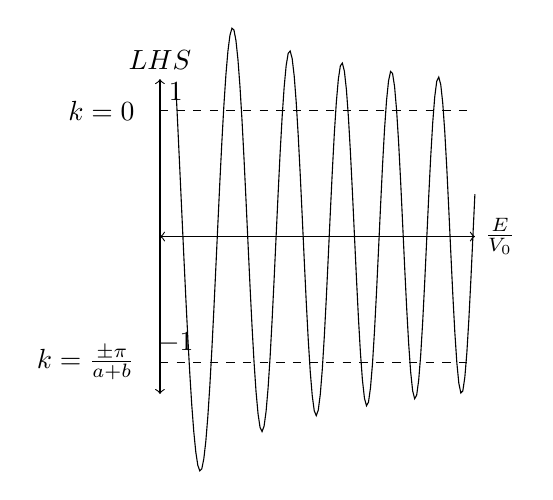
\begin{tikzpicture}[scale=0.2]
        \draw[<->] (0,0) -- (20,0);
        \node[right] at (20,0) {$\frac{E}{V_0}$};
        \draw[<->] (0,-10) -- (0,10);
        \node[above] at (0,10) {$LHS$};
        \draw[dashed] (0,8) -- (20,8);
        \node[right, above] at (1,8) {$1$};
        \node[left] at (-1,8) {$k=0$};
        \node[right, above] at (1,-8) {$-1$};
        \node[left] at (-1,-8) {$k = \frac{\pm \pi}{a+b}$};
        \draw[dashed] (0,-8) -- (20,-8);
        \draw[domain=1:20,samples=150] plot(\x, {cos(deg(\x^(1.2)))*18/\x^(0.2)});
    \end{tikzpicture}
    \caption{Plot of $k,E$}
    \label{5.12.plot}
\end{figure}

I don't know why the plot is so jumpy, but the idea is that the only physical region is where the LHS lies within the range $\pm 1$. These bands of physicality are called the band structures of crystals. We can then take the arccos of the above plot (ugh, can't draw) we can find some bands $E$ as a function of $k$. Then the allowed energies lie inside these bands.
\chapter{5/14/14 --- Conductivity in Crystals}

``This lecture will have a lot more pictures and a lot less equations.'' Uh-oh. We will begin with the picture drawn at the end of class last time, of the crystal band structure in a single dimension \ref{5.14.1D}
\begin{figure}[!h]
    \centering
    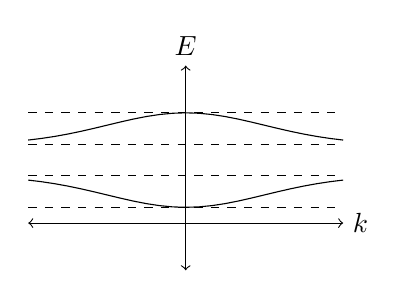
\begin{tikzpicture}[scale=0.2]
        \draw[<->] (-10,0) -- (10,0);
        \node[right] at (10,0) {$k$};
        \draw[<->] (0,-3) -- (0,10);
        \node[above] at (0,10) {$E$};
        \draw[domain=-10:10] plot(\x, {2*exp(-\x*\x/50) + 5});
        \draw[dashed] (-10,1) -- (10,1);
        \draw[dashed] (-10,3) -- (10,3);
        \draw[dashed] (-10,5) -- (10,5);
        \draw[dashed] (-10,7) -- (10,7);
        \draw[domain=-10:10] plot(\x, {-2*exp(-\x*\x/50) + 3});
    \end{tikzpicture}
    \caption{Conduction band shape. Note that only on the portions where the plot exists are allowed values of $E$. Also note that more bands exist higher up that are not depicted.}
    \label{5.14.1D}
\end{figure}

Then we can imagine populating this energy surface with electrons, the allowed states, and since electrons are Fermions we populate one electron per allowed state. Note that near the bottom of the above well we can expand $E = E_{min} + \frac{\hbar^2}{m_{eff}}$. We then see that there exists this Fermi sea of electrons near the minimum of the energy band that can move around on this global minimum of $E$.

Then what happens when we examine if we examine a pair of these bands. We can knock an electron from the bottom band up to the top band, and we can envision the ``hole'' that this produces in the bottom band as an antiparticle. We can consider then that this hole can move around too, so we can really think of it as a quasiparticle.

Since these electrons are Fermions we must use the Fermi-Dirac distribution
\begin{equation}
    f_{FD} = \frac{1}{1 + e^{(E- \mu)/kT}}
\end{equation}
which gives the average occupancy of a state of energy $E$. Note then that at low $T$ we can find $f(E > \mu - E_f) = 0, f(E < \mu - E_f) = 1$ for $E_f$ the Fermi energy, and this step function is increasingly less sharp as we increase $T$. Then we could consider our density of states function, which looks something like \ref{5.14.stateDensity}
\begin{figure}[!h]
    \centering
    \begin{tikzpicture}[scale=0.2]
        \node[right] at (6,0) {$g(E)$};
        \node[above] at (0,6) {$E$};
        \draw (5,-5) -- (5,-2);
        \draw (5,5) -- (5,2);
        \draw (0,-2) -- (0,2);
        \draw (5,2) -- (0,2);
        \draw (5,-2) -- (0,-2);
    \end{tikzpicture}
    \caption{Density of states}
    \label{5.14.stateDensity}
\end{figure}

We can then construct the average number of filled states $N(E) = g(E) f(E)$. We recall that $f(E)$ was what looked like a not-very-sharp step function. Then we can see that our $N(E)$ looks roughly like \ref{5.14.N}
\begin{figure}[!h]
    \centering
    \begin{tikzpicture}[scale=0.2]
        \draw[<->] (0,0) -- (10,0);
        \node[right] at (10,0) {$E$};
        \draw[<->] (0,-10) -- (0,10);
        \node[above] at (0,10) {$N(E)$};
        \draw[thick, domain=1:4] plot(\x, {-2*tan(17*(\x + 5))});
        \draw[thick, domain=7:10] plot(\x, {-2*tan(17*(\x + 5))});
        \draw[thick] (4,{-2*tan(17*9)}) -- (0,{-2*tan(17*9)});
        \draw[thick] (7,{-2*tan(17*12)}) -- (0,{-2*tan(17*12)});
        \draw[thick] (0,{-2*tan(17*9)}) -- (0,{-2*tan(17*12)});
    \end{tikzpicture}
    \caption{Average number of filled states as a function of energy; proportions are a bit off but $N$ vanishes where $g$ vanishes, the disallowed bands.}
    \label{5.14.N}
\end{figure}

We then see that if we compare our conductors, semiconductors, and insulators in their allowed energy levels we see that conductors have continuous energy levels, insulators have a big energy gap between allowed energy levels, and semiconductors have a small energy gap between the valence (bottom) and conduction (top) bands. 

We can also do something called doping semiconductors, which basically introduces another energy level at the Fermi level. Then there are two types of semiconductors, $N$ and $P$ type; the former has the conduction band very close to Fermi level and valence band quite far down, and the latter vice versa. Then we see that doping drops the conduction band down in $N$-type semiconductors and brings the valence band up in $P$ type semiconductors. Then in $N$ type semiconductors we can see that conduction is still carried out by electrons, but in $P$ type semiconductors since the Fermi level exchanges quite freely with the valence band it's easier to think of \emph{holes} or antiparticles carrying out the conduction.

\chapter{5/16/14 --- Quantum Hall Effect}

Recall the classical Hall Effect, where if we send currents through a $\vec{B}$ field a vertical voltage is induced. More specifically, the electrons will rotate at some $\omega_0 = \frac{qB}{mc}$ when sent through a $\vec{B}$ field.

Let's then set this up $\vec{B} = B\hat{z}$ which yields $\vec{A} = \frac{B}{2}\left( -y,x,0 \right)$. We can then plug this through our electromagnetic Hamiltonian
\begin{align}
    H &= \frac{\left( \vec{p} - \frac{q}{c}\vec{A} \right)^2}{2m} = \frac{\left( p_x + \frac{qyB}{2c}, p_y - \frac{qxB}{2c},0 \right)^2}{2m}\\
    &= \frac{\left( p_x + \frac{qyB}{2c} \right)^2}{2m} + \frac{\left( p_y - \frac{qxB}{2c} \right)^2}{2m}
\end{align}
where we assume $p_z = 0$ because we're in a flat plane. Let's then define generalized coordinates $P = p_y - \frac{qxB}{2c}, Q = \left(cp_x + \frac{qyB}{2}\right)$. so now our Hamiltonian just looks like
\begin{equation}
    H = \frac{P^2}{2m} + \frac{1}{2}m\omega_0^2Q^2
\end{equation}
with $\omega_0$ as we found earlier. Then if we compute the commutator we find $\left[ Q,P \right] = i\hbar$ which then completes the analog to the harmonic oscillator! Then we can obviously decompose this into ladder operators
\begin{align}
    H &= \left( a^\dagger a + \frac{1}{2} \right)\hbar \omega_0\\
    a &= \left( \frac{m\omega_0}{2\hbar} \right)^{1/2}Q + i\left( \frac{i}{2m\omega_0\hbar} \right)P
\end{align}
with eigenvalues of $a^\dagger a$ labelled $n \in \mathbb{R}_{\geq 0}$, called \emph{Landau Levels}. 

Then we can also define $P' = \frac{cP_x - qyB/2}{qB}$ and $Q' = P_y + \frac{qxB}{2c}$. It turns out then that $\left[ P,P' \right] = \left[ P,Q' \right] = \left[ Q,P' \right] = \left[ Q,Q' \right] = 0$. This suggests that our Hamiltonian has a few extra symmetries, because $\left[ P',H \right] = \left[ Q',H \right] = 0$, which give rise to extra degeneracies in energy levels.

Let's construct the ground state. Recall that $a\ket{0} = 0$, so let's just write out $a$ as below
\begin{align}
    a &= \left( \frac{qB}{2\hbar c} \right)^{1/2} \left[ \frac{cp_x + \frac{qyB}{2}}{qB} \right] + i\left( \frac{c}{2\hbar qB} \right)^{1/2}\left[ p_y - \frac{qxB}{2c} \right]\\
    &= \left( \frac{c}{2\hbar qB} \right)^{1/2}\left[ -i\hbar \left( \pd{}{x} + i\pd{}{y} \right) - i\left( \frac{qB}{2c} \right)(x + iy) \right]
\end{align}

It's then clear that we should go to $z = x + iy$ coordinates, and from complex analysis we know that $\pd{}{z^*} = \frac{1}{2}\left( \pd{}{x} + i\pd{}{y} \right)$. This then gives
\begin{align}
    a\ket{0} &= \left( 2\hbar \pd{}{z^*} + \frac{qB}{2c}z \right)\psi_0(z,z^*)\\
    &= 0
\end{align}

But the beauty then of complex analysis is that we can take this equation into a single variable, since $z,z^*$ are related. How do we do this? We instead proceed by ansatz $\psi_0(z,z^*) = \exp\left\{ \frac{-qB\abs{z}^2}{4\hbar c} \right\}U(z,z^*)$ which we try to get rid of the $z$ term in the ground state equation. Then we find
\begin{align}
    \left( \pd{}{z^*} + \frac{qBz}{4c} \right)\psi_0(z,z^*) &= e^{-\frac{qB\abs{z}^2}{4\hbar c}}\pd{}{z^*}U\\
    &= 0
\end{align}

We also know that the exponent is nonzero, so then we just must solve $\pd{}{z^*}U(z,z^*) = 0$ which gives $U = U(z)$. 

It turns out that if we use $\vec{A}$ in a different gauge though, that our symmetries are much more manifest. Consider $\vec{A} = Bx\hat{y}$. Then we obtain Hamiltonian
\begin{align}
    H &= \frac{p_x^2}{2m} + \frac{1}{2m}\left( p_y - \frac{qxB}{c} \right)^2\\
    &= \frac{p_x^2}{2m} + \frac{1}{2}m\omega_0^2\left[ x - \frac{p_y}{m\omega_0} \right]^2
\end{align}
but then since $H$ no longer really depends on $y$, we see that this literally looks like a coordinate shift in the Hamiltonian for a harmonic oscillator. Thus we can see this system as a harmonic oscillator just translating along the plate, translating as per $p_y$, and this $p_y$ is the origin of the degeneracy.

Lastly, we can discuss the degeneracy for Landau level in a finite $2d$ surface that is $L_x \times L_y$ dimensions? Then we know that $P_y= \frac{2\pi \hbar}{L_y}n$ with $n \in \mathbb{Z}$. We also note that since $0 \leq x_0 \leq L_x$ that $0 \leq N < \frac{m\omega_0 L_x L_y}{2\pi \hbar}$ (if we join our $x_0 = x - \frac{p_y}{m\omega_0}$ translation from our above Hamiltonian). But then we note that $N \leq \frac{BL_xL_y}{\Phi_{q}}$ with $\Phi_q$ the flux quantum! Therefore $N$ must be less than the number of flux quanta though the plate.
\chapter{5/19/14 --- Dirac Equation}

We note that the SE has a very asymmetric form when it comes to time and space, as we recall
\begin{equation}
    i\hbar \pd{}{t}\ket{\psi} = -\frac{\hbar^2}{2m} \ptd{}{x}\ket{\psi}
\end{equation}
where we neglect the potential to emphasize the fact that $x,t$ \emph{should} be on completely equal footing while they're obviously not. We want to turn these onto super-equal footing, and the only way to fully do this is through QFT, though what we do now is going to be a consistent buildup.

Recall from relativity that $E = \sqrt{m^2c^4 + p^2c^2}$. We typically expand in $p \ll mc$ so that $E = mc^2 + \frac{p^2}{2m} + O(p^4)$. There is then a very clear ansatz for the SE if we consider $H\ket{\psi} = E\ket{\psi}$, namely
\begin{equation}
    H = \sqrt{m^2c^4 + p^2c^2} = \sqrt{m^2c^4 - \hbar^2 c^2 \ptd{}{x}}= i\hbar \pd{}{t}
\end{equation}
where we define the square root of the operator as the series expansion. It is still clear that we don't have symmetry though! The issue arises from the square root, because we have the problem of which root to take. If we were to square both sides, we would arrive at
\begin{align}
    H^2 = m^2c^4 - \hbar^2c^2 \ptd{}{x} &= -\hbar^2 \ptd{}{t}\\
    \left(\ptd{}{t} - c^2\ptd{}{x} + \frac{m^2c^4}{\hbar^2}\right)\phi &= 0
\end{align}

This looks much more symmetric! This is the \emph{Klein-Gordon Equation}. The partials are obviously Lorentz invariant. 

Note that $\phi$ isn't exactly our wave equation though. Two reasons
\begin{itemize}
    \item This is a second-order ODE, which means we need two ICs, $\phi,\phi'$, not characteristic of our usual ``get the wavefunction and propagate it.''
    \item Implies negative energy solutions exist! This is because we squared both sides, meaning we also introduce the negative root. Because the negative root exists inherently as a solution, this means our equation is a bit dubious (i.e. it's dubious beyond just ``throw out the negative solutions'')
\end{itemize}

We can see these negative energies by examining a solution of form $\phi \sim e^{i(kx - \omega t)}$, which through the Klein-Gordon equation produces $\omega(k) = \pm \sqrt{c^2k^2 + \frac{m^2c^4}{\hbar^2}}$. This is bad though, because particles would then tend to states of infinite $k$ with the negative roots! One possible solution is to fill all the lower energy levels with Fermions, but this still doesn't work for Bosons.

Hm. Let's go back to $H^2 = m^2c^4 + p^2c^2$. Let's examine this instead as $H^2 = m^2c^4 + \left( p_x^2 + p_y^2 + p_z^2 \right)c^2$. We then want to take the square root of this equation, so let's write some ansatz $H = \beta mc^2 + c(\alpha_xp_x + \alpha_yp_y + \alpha_zp_z) = \beta mc^2 + c\vec{\alpha} \cdot \vec{p}$. Plugging this in we have
\begin{align}
    H^2 =& c^2\left[ \alpha_x^2p_x^2 +\alpha_y^2p_y^2+\alpha_z^2p_z^2 \right] + \beta^2 m^2c^4 + \left[ c^2 p_yp_y(\alpha_x\alpha_y+ \alpha_y\alpha_x) + c^2 p_yp_y(\alpha_z\alpha_y+ \alpha_y\alpha_z) + c^2 p_yp_y(\alpha_x\alpha_z+ \alpha_z\alpha_x) \right]\nonumber\\
    &{}+ mc^3\left[p_x(\alpha_x\beta + \beta \alpha_x) + p_y(\alpha_y\beta + \beta \alpha_y) + p_z(\alpha_z\beta + \beta \alpha_z)\right]
\end{align}

We write it this complicated-ly because we anticipate that $\alpha_i, \beta$ are not numbers, but matricies! Note that the above equations imply $\alpha_x^2 = \alpha_y^2 = \alpha_z^2 = \beta^2 = 1$, but at the same time $\left\{ \alpha_i, \alpha_j \right\} = 2\delta_{ij}, \left\{ \alpha_i, \beta \right\} = 0$ the anticommutators. We note that this is eerily reminiscent of the Pauli matricies.

We will guess that $\alpha_i, \beta$ are $4\times4$ matricies, in $2\times2$ blocks. We will write down then that
\begin{align}
    \alpha_i &= \begin{bmatrix} 0 & \sigma_i \\ \sigma_i & 0 \end{bmatrix} & \beta &= \begin{bmatrix} \mathbb{I} &0 \\ 0 & -\mathbb{I} \end{bmatrix} 
\end{align}
for $\mathbb{I}$ the $2\times2$ identity and $\sigma_i$. Thus, our full fledged Dirac equation looks like
\begin{align}
    i \hbar \pd{}{t}\ket{\psi} &= H\ket{\psi} = \left( c\vec{\alpha} \cdot \vec{P} + \beta mc^2 \right)\ket{\psi}
\end{align}

We finally have the derivatives all on the same footing!
\chapter{5/21/14 --- Finishing Dirac Equation, Classical field theory}

Recall that we had established the Dirac equation
\begin{equation}
    i\hbar \pd{}{t}\ket{\psi} = (c\vec{\alpha} \cdot \vec{P} + \beta mc^2)\ket{\psi}
\end{equation}

If we want to compute this then for EM case, we will send $\vec{P} \to \vec{P} - \frac{q}{c}\vec{A} = \vec{\Pi}$ some canonical momentum for EM, which takes us to
\begin{equation}
    i\hbar \pd{\psi_E}{t} = E\psi_E = \left( c\vec{\alpha} \cdot \vec{\Pi} + \beta mc^2 \right)\Psi_E
\end{equation}
where we will write $\psi_E = \left( \chi, \Phi \right)^T$ with each of $\chi, \Phi$ two-vectors. Let's now write this out for stationary $\psi_E$
\begin{align}
    \left(E - c\vec{\alpha} \cdot \vec{\Pi} - \beta mc^2\right)\psi_E &= 0\\
    \begin{bmatrix} E-mc^2 & -c \vec{\sigma} \cdot \vec{\Pi} \\ -c\vec{\sigma} \cdot \vec{\Pi} & E + mc^2 \end{bmatrix} \begin{bmatrix} \chi \\ \Phi \end{bmatrix} &= \begin{bmatrix} \left( E - mc^2\right) \chi - c\vec{\sigma} \cdot \vec{\Pi} \Phi \\ \left( E + mc^2\right) \Phi - c\vec{\sigma} \cdot \vec{\Pi} \chi \end{bmatrix} = \begin{bmatrix} 0\\0 \end{bmatrix} \label{5.12.other}
\end{align}
which gives us via the second component
\begin{equation}
    \Phi = \frac{c\vec{\sigma} \cdot \vec{\pi}}{E + mc^2}\chi
\end{equation}

Let's then expand $E + mc^2 = 2mc^2 + E_s$ with $E_s$ the Schrodinger energy. We can examine the scale of the prefactor. We note that $p \sim mv$, so the expression goes like $\Phi = O\left( \frac{v}{c} \right)\chi$. Just to get some idea of what the terms' scales look like.

Let's now examine the first component of \eqref{5.12.other}, which yields
\begin{align}
    E_s\chi &= c\vec{\sigma} \cdot \vec{\Pi}\Phi = \frac{c\left( \vec{\sigma} \cdot \vec{\Pi} \right)c\left( \vec{\sigma} \cdot \vec{\Pi} \right)\hat{}}{E + mc^2}\\
    &\approx \frac{1}{2m} \left( \vec{\sigma} \cdot \vec{\Pi} \right)\left( \vec{\sigma} \cdot \vec{\Pi} \right) \chi
\end{align}
where we go ahead and substitute $E + mc^2 \approx 2mc^2$. We now plug in $\left( \vec{\sigma}\cdot \vec{A} \right)\left( \vec{\sigma}\cdot \vec{A} \right) = \left( \vec{A} \cdot \vec{B} \right)\mathbb{I} + i\vec{\sigma} \cdot \left( \vec{A} \times \vec{B} \right)$ identity for spin matricies, and we obtain
\begin{equation}
    E_s\chi = \frac{1}{2m}\left[ \vec{\Pi}^2 - \frac{q\hbar}{c}\vec{\sigma} \cdot \vec{B} \right]\chi
\end{equation}
using that $\vec{\Pi} \times \vec{\Pi} = \frac{iq\hbar}{c}\vec{B}$. The surprising thing about this is that through our formalism we've found the next order behavior of the Dirac equation to have an extra coupling of the spin to the magnetic field $\vec{\mu} \cdot \vec{B}$ with $\mu = \frac{q\hbar \sigma}{2mc}$. This is a non-relativistic effect that falls out of the relativistic formulation! (This is I believe the explanation behind the $g=2$ magnetic moment of the electron, hinted at way long ago.) 

Note that we haven't yet discussed whether $\chi$ is a wavefunction or probability amplitude or whatever, let's do that now. Let's first turn off $\vec{B}$ field and consider only the $\vec{\Pi} = \vec{P}$ term. This gives us in the full (not non-relativistic limit) form
\begin{align}
    \chi &= \frac{c^2}{E^2 - m^2c^4}(\vec{\sigma} \cdot \vec{P})(\vec{\sigma} \cdot \vec{P})\chi\\
    &= \frac{c^2p^2}{E^2 - m^2c^4} \chi
\end{align}
then our fraction must be equal to $1$ which still produces $E = \pm\sqrt{m^2c^4 + p^2c^2}$; why do we still have negative energies?? Oops. Dirac here proposes the \emph{Dirac sea}, which is a sea of electrons that fills up the negative energies. This is discredited now.

We now know the correct explanation is that $\chi, \Phi$ are not probability amplitudes/wavefuctions, in either the Dirac or Klein-Gordon equations. They are what we call \emph{classical fields}. We can see this by noting that the equations we've found do not treat $\Phi, \chi$ as complex varibales; indeed we could treat them as completely real and we'd still maintain the result we have right now! Probabilities must be complex though, at some level, so we know these couldn't have been complex.

We figure out what these are by considering the following little table\ref{tab:5.21.organizetable}
\begin{table}
    \centering
    \begin{tabular}{l|l|l|}
        &Particles & fields\\[10pt]\hline
        Classical & $x(t), \dot{x}(t)$ (not usually Lorentz invariant) & $\vec{E}(x,t), \vec{B}(x,t)$ (Lorentz invariant)\\[10pt]\hline
        Quantum & $\psi(x,t)$ (not Lorentz invariant)& ??
    \end{tabular}
    \caption{Table of what we know so far}
    \label{tab:5.21.organizetable}
\end{table}

We thus see that $\vec{A}$ is a classical field though, so it is then evident that our $\phi, \psi$ in our Klein-Gordon and Dirac Equations must be operating on classical fields! Then we know that $\phi, \psi$ are scalar fields rather than wavefunctions. 

It is then pretty natural to think back to our Table \ref{tab:5.21.organizetable} and realize that our missing link is QFT!

To figure out how to get to QFT, it's easiest to first figure out how classical field theories arise. EM is already one classical field theory we're familiar with; let's consider phonons instead. Phonons are sound waves, which are generated by particles bouncing against one another. We'll try to derive the Klein-Gordon equation from some simple phonon model. Consider a 1D lattice of particles as just many coupled balls and springs, infinite HOs. 

Call $a$ the equilibrium distance between masses in our lattice. Then our Lagrangian looks like
\begin{equation}
    L = \sum\limits_{-N/2}^{N/2} \frac{1}{2}m\dot{x}_n^2 - \frac{k}{2}\left( x_{n+1} - x_n - a \right)^2
\end{equation}

Define then the equilibrium positions $\bar{x}_n = na$ and $x_n(t) = \bar{x}_n + y_n(t)$ then we can just rewrite this as 
\begin{equation}
    L = \sum\limits_{-N/2}^{N/2} \frac{1}{2}m\dot{y}_n^2 - \frac{k}{2}\left( y_{n+1} - y_n \right)^2
\end{equation}

Now we take $a \to 0$, but this will have to wait till next class! Basially we will take $y_n(t)$ and replace it with $y(t,x)$ such that $x = na$ with $n \in [0,N]$ as $N \to \infty$ naturally. 

\chapter{5/23/14 --- Phonons}

Third to last Cliff lecture, nooooo. Too many good profs being left behind.

Recall that we had phonons each labelled by some coordinate $x_n$ with mass $m$ connected with springs at some equilibrium distance $a$ and spring constant $k$. We then wrote down the coordinates that subtracted out the equilibrium position, so that the Lagrangian looked like
\begin{equation}
    L = \sum\limits_{}^{}\frac{1}{2} m\dot{y}_n^2 - \frac{k}{2}\left( y_{n+1} - y_n \right)^2
\end{equation}

We then take the continuum limit, so $a\to 0, N \to \infty$ such that $Na = L$. We then also replace $n \to x$ so that $na = x$. We then substitute $y_n \to y(x), y_{n+1} - y_n \to a \pd{}{x}y(x)$, and replace the sum with an integral so that our Lagrangian becomes
\begin{equation}
    L = \int\limits_{-L/2}^{L/2} \frac{1}{2}\frac{m}{a}\dot{y}^2 - \frac{ka}{2}\left( \pd{y}{x} \right)^2\;dx
\end{equation}
or defining $y\sqrt{\frac{m}{a}} = \phi$ we obtain simple form
\begin{equation}
    L = \int\limits_{}^{}dx\;\frac{1}{2}\dot{\phi}^2 - \frac{1}{2}\left( \frac{ka^2}{m} \right)\left( \pd{\phi}{x} \right)^2
\end{equation}

We could obviously upgrade to 3D just by taking a triple integral instead, and going from $x,y,z$. We will do so right now, as below (define $v^2 = \frac{ka^2}{m}$)
\begin{equation}
    S = \int\limits_{}^{}L\;dt = \int\limits_{}^{}dt\;d^3x\left[ \frac{1}{2}\dot{\phi}^2 - \frac{1}{2}v^2\left( \vec{\nabla}\phi \right)^2 \right]
\end{equation}

Note that we are suddenly integrating over all spacetime now, so this will be convenient for relativity! But in any case, that's just a preview; the above is the action for a classical field describing a phonon.

Then we go to the Newtonian EOM $m\ddot{y}_n - k\left( y_{n+1} - y_n \right) + k(y_n - y_{n-1}) = 0$ and take this to the continuum limit and we find that 
\begin{equation}
    \ddot{\phi} - v^2\nabla^2\phi = 0
\end{equation}

This is actually the Klein-Gordon equation, but $\phi$ is not nearly a wavefunction! We know also that this is the wave equation, which we can solve (in the 1D case) to obtain general solution form
\begin{equation}
    \phi(x,t) = f_R(x-vt) + f_L(x + vt)
\end{equation}
(thankfully we are learning this in ACM95c, PDEs, right now! Not) which we can add a self-interaction term (in Lagrangian in the way of a $my_n^2$ term) to obtain
\begin{equation}
    \ddot{\phi} - \nabla^2 \phi + m^2\phi = 0
\end{equation}

Now let's try to solve this non-wave equation with the wave equation ansatz and see what happens, $\phi = e^{i(\vec{k} \cdot \vec{x} - \omega t)}$ which gives us $-\omega^2 + k^2 + m^2 = 0$ and yields solutions $\omega = \pm \sqrt{k^2 + m^2}$. 

So now we have some $\phi$ field and we can expand in terms of the two solutions, or in other words we can write down general solution
\begin{equation}
    \phi(x,t) = \int \left[\frac{d^3k}{f(k)}\right]\left[ a(\vec{k})e^{i(\vec{k} \cdot \vec{x} - i\omega_kt)} + a(\vec{k})^* e^{-i\vec{k} \cdot \vec{x} + i \omega_k t} \right]
\end{equation}
where we impose the condition that $\phi(x,t)$ is real, so we just sum over possible solutions and their complex conjugates (also okay solutions), and we can insert the real function $f(k)$ to anticipate future results\dots

Now let's go to quantum fields. How would we turn $\phi$ into a quantum mechanical object? Well, typically we just smash all variables of $\phi$ into operators and define the Hilbert space. Here, we will do this more formally, via \emph{second quantization}. This is a terrible name because it's just a historical artifact of the fact that people thought the Klein-Gordon equation was aleady quantized so we need to re-quantize $\phi$, though we now know that $\phi$ is obviously a classical object. But basically, second quantization means that we will quantize a classical field.

How do we do this then? ``It's actually very simple,'' we will just turn $a(\vec{k})$ into a lowering operator, and $a^*$ into a raising operator, obviously. But now, since they are indexed by a continuum $\vec{k}$, we wonder what happens when we examine $\left[ a(\vec{k}, a(\pvec{k}) \right]$? This turns out to be $0$. And naturally, $[a(\vec{k}), a^\dagger(\pvec{k})] \sim \delta^3(\vec{k}  - \pvec{k})$, so they commute unless they're the same $\vec{k}$. 

Then we can interpret $\phi(x,t)$ as an infinite tower of harmonic oscillators labelled by the continuum $\vec{k}$, each of which is independent (their ladder operators commute). So we've decomposed the phonon system into a set of all modes it can exhibit, and we quantize each of these modes! We will work this more carefully.

But first, let's examine the Lorentz invariance of $\phi(x,t)$ via first determining $f(k)$ in our definition. We will require the measure $\frac{d^3k}{f(\vec{k})}$ to be Lorentz invariant. Let's choose $f(\vec{k}) = 2\omega_k = 2\sqrt{k^2 + m^2}$. Then our measure is secretly Lorentz invariant despite only seeming to have three dimensions of space; we'll examine this by looking to the integral $\int d^4\mathbf{k} = \int d^3\vec{k}\; dk_0$. We must somehow get rid of one of the $k$s, so we will examine the integral
\begin{equation}
    \int d^4\mathbf{k}\; \delta\left( (k_0^2 - \vec{k}^2) - m^2 \right)\Theta(k_0)
\end{equation}
with $\Theta$ the Heaviside step. We then note that the first two terms that are manifestly invariant, and the third term restricts us to positive $k_0$ (note that since we have $\vec{k}$, the 4-vector $(k_0, \vec{k})$ corresponds to an energy-momentum pair, so we are effectively picking out positive energy, since positivity of energy is Lorentz invariant). We can then evaluate out this integral
\begin{align}
    \int d^4\mathbf{k}\; \delta\left( (k_0^2 - \vec{k}^2) - m^2 \right)\Theta(k_0) &= \int d^3\vec{k} dk_0 \Theta(k_0)\left[ \frac{\delta(k_0 - \omega_k)}{2k_0} + \frac{\delta(k_0 + \omega_k)}{2k_0} \right]
\end{align}

The step function then eliminates the second term, and we find this to be all equal to $\int \frac{d^3\vec{k}}{2\omega_k}$ which shows that our chosen measure is Lorentz invariant! Then it is clear that if we had thrown any function of $\vec{k}$ in front of the integral, the whole integral remains Lorentz invariant (in front of the $\int d^4\mathbf{k}$ integral), so thus we see that $\phi$ is actually Lorentz invariant! We can see this by writing $\phi$ as
\begin{equation}
    \phi(x,t) = \int d^4\mathbf{k} \delta\left( \mathbf{k}^2 - m^2 \right)\Theta(k_0)\left[ a(\vec{k}) e^{-i \mathbf{k} \cdot \mathbf{x}} + a(\vec{k})^\dagger e^{i \mathbf{k} \cdot \mathbf{x}} \right]
\end{equation}

This is super obviously Lorentz invariant now! We just need to figure out how the ladder operators transform. (I denote 4-vectors boldface)

\chapter{5/28/14 --- QFT}

Recall that we had arrived at our classical, Lorentz-invariant field
\begin{equation}
    \phi(\vec{x},t) = \left[ \frac{d^3k}{\left( 2\pi \right)^32\omega_k} \right]\left[ a(\vec{k}) e^{-ikx} + a^*(\vec{k})e^{ikx}\right]\label{5.28.phi}
\end{equation}

Let's then define a Lagrangian density $S = \int \mathcal{L}\; dt\; d^3x$. whuch for us looks like
\begin{equation}
    S = \int d^4x \frac{1}{2}\dot{\phi}^2 - \frac{1}{2}\left( \vec{\nabla}\phi \right)^2 - \frac{m^2\phi^2}{2}
\end{equation}

Then if we want to go from the Lagrangian to the Hamiltonian we take the Legendre transform. So if we look at the Lagrangian density above in terms of $q_i, \dot{q_i}$, then we can find a canonical momentum. We then wonder what the analog of $\vec{\nabla}\phi$ is, and since it's just dependent on the positions of nearest neighbors we note that it should transform like $q$ and not $\dot{q}$. 

Then we can define $\pi(x,t) = \pd{L}{\dot{\phi}(x,t)} = \dot{\phi}$, which is a bit odd since there's no mass but we're okay with this. Then we define $\mathcal{H} = \pi\dot{\phi} - \mathcal{L}$ some Hamiltonian density, which computes to be
\begin{equation}
    H = \int \mathcal{H}\; d^3x = \int d^3x \left[ \frac{1}{2}\dot{\phi}^2 + \frac{(\vec{\nabla}\phi)^2}{2} + \frac{1}{2}m^2\phi^2 \right]
\end{equation}

This shows that if we have a field with high values or high time/position derivatives then this is high energy, which makes a lot of sense.

Now we want to plug in our $\phi$ from \eqref{5.28.phi} to this Hamiltonian. We will recall that $\int d^3x e^{-i\vec{k\cdot \vec{x}}}e^{-i\pvec{k} \cdot \vec{x}} = \delta^3(\vec{k} + \pvec{k})(2\pi)^3$, so a lot of delta functions pop up and we get our Hamiltonian to be
\begin{equation}
    H = \int d^3x\; \frac{1}{2}\omega_k\left( a^\dagger(\vec{k})a(\vec{k}) + a(\vec{k}) a^\dagger(\vec{k}) \right)
\end{equation}

This gives us that our Hamiltonian is defining a set of HOs with different $\omega_k$. Note that this must also be Lorentz invariant, though it's not quite as obvious, because it started with a Lorentz-invariant Lagrangian. Then we want to quantize these guys, so we use $[a(\vec{k}), a^\dagger(\pvec{k})] = (2\pi)^3(2\omega_k)\delta^3(\vec{k} - \pvec{k})$ and obviously $[a(\vec{k}), a(\pvec{k})] = 0$ and for $a^\dagger$. However, then we note that plugging in this commutator to the Hamiltonian yields something like
\begin{equation}
    H = \int d^3k\; \frac{1}{2}\omega_k \left( 2a^\dagger(\vec{k})a(\vec{k}) + (2\pi)^3(2\omega_k)\delta^3(0)\right)
\end{equation}
which is an infinity! QFT is infamous for its infinities, and in our case this is just a zero point energy that we can ignore. The only force in the world that cares about absolute energies is gravity, and it remains a puzzle today why gravity doesn't see this delta function either; big unsolve problem in physics. It turns out that many infinities in QFT we can throw out, which gives rise to its somewhat dubious reputation.

We can also give $\phi,\pi$ commutation relations, which is just $\left[ \phi(\vec{x}), \pi(\pvec{x}) \right] = i\delta^3(\vec{x} - \pvec{x})$ and of course $\left[ \phi(\vec{x}), \phi(\pvec{x}) \right] = \left[ \pi(\vec{x}), \pi(\pvec{x}) \right] = 0$.

Let's now define $\ket{0}$ the true vacuum state, such that $a(\vec{k})\ket{0} = 0$ for any $\vec{k}$, and $\dotp{0}{0} = 1$. We can also interpret a ket $\ket{\vec{k}_i} = a(\vec{k}_i)\ket{0}$ which is a single particle with a wavenumber $\vec{k}_1$. Then naturally $\ket{\vec{k}_i, \vec{k}_j} = a^\dagger(\vec{k}_i)a^\dagger(\vec{k}_j)\ket{0}$ is a state with two particles.

Then we can look at what happens when $\dotp{\vec{k}_1}{\vec{k}_2}$, which is just
\begin{align}
    \dotp{\vec{k}_1}{\vec{k}_2} &= \bra{0}a(\vec{k}_1)a^\dagger(\vec{k}_2)\ket{0}\\
    &= \bra{0}a^\dagger(\vec{k}_2)a(\vec{k}_1) + (2\pi)^32\omega_{k_1} \delta^3(\vec{k}_1 - \vec{k}_2\ket{0}\\
    &= \dotp{0}{0}(2\pi)^32\omega_{k_1} \delta^3(\vec{k}_1 - \vec{k}_2)\\
    &= (2\pi)^32\omega_{k_1} \delta^3(\vec{k}_1 - \vec{k}_2)
\end{align}
which is good since $\int d\tilde{k}_1 \dotp{\vec{k}_1}{\vec{k}_2} = 1$. 

Note also that $\dotp{k_2}{k_1,. k_2} = 0$, or more generally particles are not created spontaneously since the states are orthogonal. This isn't very interesting though, and the obvious solution is to go to a more interesting theory. In our case, we can easily add terms to our Lagrangian density such as $\lambda \phi^4$, which gives new ways to connect states other than just free propagation.
\chapter{5/30/14 --- QFT explorations!}

Recall that our Lagrangian and our corresponding Hamiltonian
\begin{align}
    L_0 &= \int d^4\mathbf{x} \mathcal{L} = \int d^4\mathbf{x} \left( \frac{1}{2}\dot{\phi}^2 - \frac{1}{2}\left( \vec{\nabla}\phi \right)^2 - \frac{1}{2}m^2\phi^2 \right)\\
    H_0 &= \int d^3x \mathbf{H} = \int d^3x \left( \frac{1}{2}\dot{\phi}^2 + \frac{1}{2}\left( \vec{\nabla}\phi \right)^2 + \frac{1}{2}m^2\phi^2 \right)
\end{align}

Now let's add some $V(\phi)$ that goes with higher powers of $\phi$, so that $L = L_0 - V$ and $H = H_0 + V$. Thisis what produces the rich dynamics of the world!

We must now figure out what picture we're in. Let's now produce our quantum field 
\begin{align}
    \phi(\vec{x},t) &= \int d^4\mathbf{k}\left( a(\vec{k}) e^{-i\left( \vec{k} \cdot \vec{x} - \omega t \right)} + a^\dagger(\vec{k}) e^{i\left( \vec{k} \cdot \vec{x} - \omega t \right)}\right)
\end{align}

Note that $\phi$ has a $t$ dependence, and since the Schr\"odinger picture operators are constant in time, this probably isn't a Schr\"odinger picture operator. If we rewrite this while grouping the time dependences we find
\begin{align}
    \phi(\vec{x},t) &= \int d^4\mathbf{k}\left[ \left( a(\vec{k})e^{-i\omega t} \right)e^{i\vec{k} \cdot \vec{x}} + \left(a^\dagger(\vec{k})e^{i\omega t}\right)e^{-i\vec{k} \cdot \vec{x}} \right]
\end{align}
and then we see that the operator is undergoing some sort of unitary transformation, which seems then to look like $\phi(\vec{x},t) = U_0(t)\phi(\vec{x},0) U_0^\dagger(t)$ with $U_0 = e^{-iH_0t}$ (I'm not quite sure why it's $H_0$ as opposed to say $H$; I don't think I missed anything\dots), so we see that $\phi$ is in the Heisenberg picture. 

However, if we think back carefully we recall that in the interaction picture we write $H = H_0 + H_1$ and conjugate $H_0$ with propagator and perturb with $H_1$. In our case, we see that since our field is being conjugated by the propagator we see that this is also an interaction picture field; the two pictures are the same for the interaction-less case.

If we then want to compute transition amplitudes by introducing some sort of interaction (which will be $V(\phi)$), we can look into the usual expression $\bra{f}u(t_f, t_i)\ket{i} = \mathcal{T}_{if}$ with
\begin{align}
    U(t_f,t_i) &= 1 + (-i)\int\limits_{t_i}^{t_f}dt_1\;H_1(t_1) + (-i)^2 \int\limits_{t_i}^{t_f}\int\limits_{t_{i}}^{t_1}dt_1\;dt_2\;H_1(t_1)H_1(t_2) +\dots
\end{align}
the usual perturbation theory expansion. We will evaluate/simplify this expression using \emph{time ordering}. Physically, it means that instead of integrating each integral separately and summing them we will order the entire expression in time and then integrate. So for example
\begin{align}
    \int\limits_{t_i}^{t_f}dt_1\int\limits_{t_i}^{t_1}dt_2\dots \int\limits_{t_i}^{t_{n-1}}dt_n\;H_1(t_1)\dots H_1(t_n) = \frac{1}{n!}\int\limits_{t_i}^{t_f}dt_1\int\limits_{t_i}^{t_f}dt_2\dots T\left[ H_1(t_1)\dots H_1(t_n) \right]
\end{align}
with $T[\Omega_1(t_1)\Omega_2(t_2)]$ defined as the time-ordering operator
\begin{align}
    T\left[ \Omega_1(t_1)\Omega_2(t_2) \right] =
    \begin{cases}
        \Omega_1\Omega_2 & t_1 > t_2\\
        \Omega_2 \Omega_1 & t_1 < t_2
    \end{cases}
\end{align}

Then it turns out that the full propagator gives an absurdly clean expression
\begin{align}
    U(t_f, t_i) = T\left[ \exp\left( -i \int\limits_{t_i}^{t_f}dt\;H_1(t) \right) \right]
\end{align}

This is the central tenet of QFT; Feynman diagrams just come from expanding out the exponential. We can also define the \emph{S-matrix} $S = U(\infty, -\infty)$ also very famous in QFT. We also note that $U$ is Lorentz invariant because $\mathcal{H}_1$ the Hamiltonian density is Lorentz invariant, which means that $H_1(t) = \int d^3x \mathcal{H}_1(t)$ plugged into above is Lorentz-invariant sort of integral; we can write this down
\begin{align}
    S = T\left[ \exp\left( -i \int\limits_{-\infty}^{\infty}dt d^3x\;\mathcal{H}_1(\vec{x},t) \right) \right]
\end{align}

Then we wonder whether $T$ is a Lorentz invariant sort of operation. We intuit that since two causally related events will always have the same ordering, there should be a very clean answer on whether this clunky, messy $T$ operator is Lorentz invariant. 

Let's examine this more carefully. In our usual spacetime diagram in \ref{5.30.STdiag} we have
\begin{figure}[!h]
    \centering
    \begin{tikzpicture}[scale=0.2]
        \draw[<->] (-10,0) -- (10,0);
        \node[right] at (10,0) {$x$};
        \draw[<->] (0,-10) -- (0,10);
        \node[above] at (0,10) {$t$};
        \draw[dashed] (-10,-10) -- (10,10);
        \draw[dashed] (-10,10) -- (10,-10);
        \filldraw (0,0) circle(10pt);
        \node[below] at (0,0) {$y$};
        \filldraw (3,5) circle(10pt);
        \node[below] at (3,5) {$x$};
        \filldraw (5,3) circle(10pt);
        \node[below] at (5,3) {$x'$};
    \end{tikzpicture}
    \caption{Space time diagram. Note that $x$ is timelike separated and $x'$ is spacelike separated.}
    \label{5.30.STdiag}
\end{figure}
then we recall that the spacelike/timelike critereon is that $(x - y')^2 < 0$ while $(x-y)^2 > 0$. Then we note that the time ordering operator \emph{cannot} be Lorentz Invariant for spacelike times.

{\em \small Sorry, I think my notes are a bit garbled from here forwards\dots I've tried to reinterpret/clean them up to some degree in the Ph125cStudySession.pdf notes}

What then is the resolution for these cases, since we obtain a contradiction of relativity with QM here? We demand instead that $\left[ H_1(x), H_1(y) \right] = 0$ at space like separations, which means that in the time ordering operator no longer actually \emph{does anything}, or becomes the identity operator, in spacelike separations and so since the identity is Lorentz Invariant we resolve this contradiction. Then if we demand $H_1(x) = f(\phi(x))$ then we thus see that all such QFT theories are saved, because $\left[ \phi(x), \phi(y) \right] = 0, (x-y)^2 < 0$ (this doesn't seem evident, but we talk about that immediately next). This is also why we added $V(\phi)$ instead of arbitrary terms, because our $H_1$ still holds. Thus we see that causality forces a lot of the things that we've used so far!

What then is $\left[ \phi(x), \phi(y) \right]$? This is just (sorry, we've been dropping 4-vector things in lecture, but it should be evident that $x,y$ were 4-vectors)
\begin{align}
    \left[ \phi(x), \phi(y) \right] &= \left[ \int d^4\mathbf{k}\left( a(\vec{k})e^{-ikx} + a^\dagger(\vec{k})e^{i\mathbf{k}\mathbf{x}} \right), \int d^4\mathbf{p}\left( a(\vec{p})e^{-i\mathbf{p} \cdot \mathbf{y}} + a^\dagger(\vec{p})e^{i\mathbf{p} \cdot\mathbf{y}} \right) \right]\\
    &= \int d\mathbf{k} d\mathbf{p}\left( \left[ a(\vec{k}), a^\dagger(\vec{p}) \right]e^{-ikx}e^{ipy} + \left[ a^\dagger(\vec{k}),a(\vec{p}) \right]e^{ikx}e^{-ipy} \right)\\
    &\sim \int dk\; dp\left( \delta^3(\vec{k} - \vec{p})e^{-ikx + ipy} - \delta^3(\vec{k} - \vec{p}) e^{ikx - ipy} \right)\\
    &\sim \int dk\left[ e^{-ik\left( x-y \right)} - e^{ik\left( x-y \right)} \right]
\end{align}

Then only when $(x-y)^2 < 0$ then we can find a frame in which $x-y \to y-x$, so we see that the commutator vanishes exactly when $(x-y)^2 < 0$. This then shows that as long as the Hamiltonian is constructed only out of field operators $\phi$ then the full S-matrix will be Lorentz-invariant because the $T$ operator is Lorentz invariant.

It makes sense that this commutator vanishes for spacelike domains though, because if Alice makes a measurement using $\phi(x)$ and Bob at $\phi(y)$ then if the measurements didn't commute causality would be violated. So the fact that all of QFT hinges around these $\phi$ and that these $\phi$ obey this commutation relation shows that causality is a consquence of QFT (not exactly his wording, but that's how I feel about this)!

We can lastly discuss tachyons shortly, which looks actually like $E = \sqrt{p^2 - m^2}$, superluminal travel. Then our Lagrangian density would something like $L = \frac{1}{2}\dot{\phi}^2 - \frac{1}{2}(\vec{\nabla}\phi)^2 + \frac{1}{2}m^2\phi^2$, the sign change, then things would get super wacky. For example, $H = \dots - \frac{1}{2}m^2\phi^2$ and we see that the potential falls off infinitely! This means that there is no longer any ground state, no vacuum, and this theory royally sucks (is ``sick'' according to Cliff).

But then if we add more terms to our potential, such as $L' = L - \lambda \phi^4$ then our potential would look like a quartic sort of thing, and so the vacuum is recovered; this is the context in we should discuss tachyons. Last note, the Higgs Boson is actually a field that obeys a tachyonic sort of potential (this last quartic thing) which is why the universe is a little bit weirder than we expect? Something like that, but just a little thing. Congrats on finishing Ph125!

\end{document}
